\documentclass[twoside]{book}

% Packages required by doxygen
\usepackage{fixltx2e}
\usepackage{calc}
\usepackage{doxygen}
\usepackage[export]{adjustbox} % also loads graphicx
\usepackage{graphicx}
\usepackage[utf8]{inputenc}
\usepackage{makeidx}
\usepackage{multicol}
\usepackage{multirow}
\PassOptionsToPackage{warn}{textcomp}
\usepackage{textcomp}
\usepackage[nointegrals]{wasysym}
\usepackage[table]{xcolor}

% Font selection
\usepackage[T1]{fontenc}
\usepackage[scaled=.90]{helvet}
\usepackage{courier}
\usepackage{amssymb}
\usepackage{sectsty}
\renewcommand{\familydefault}{\sfdefault}
\allsectionsfont{%
  \fontseries{bc}\selectfont%
  \color{darkgray}%
}
\renewcommand{\DoxyLabelFont}{%
  \fontseries{bc}\selectfont%
  \color{darkgray}%
}
\newcommand{\+}{\discretionary{\mbox{\scriptsize$\hookleftarrow$}}{}{}}

% Page & text layout
\usepackage{geometry}
\geometry{%
  a4paper,%
  top=2.5cm,%
  bottom=2.5cm,%
  left=2.5cm,%
  right=2.5cm%
}
\tolerance=750
\hfuzz=15pt
\hbadness=750
\setlength{\emergencystretch}{15pt}
\setlength{\parindent}{0cm}
\setlength{\parskip}{3ex plus 2ex minus 2ex}
\makeatletter
\renewcommand{\paragraph}{%
  \@startsection{paragraph}{4}{0ex}{-1.0ex}{1.0ex}{%
    \normalfont\normalsize\bfseries\SS@parafont%
  }%
}
\renewcommand{\subparagraph}{%
  \@startsection{subparagraph}{5}{0ex}{-1.0ex}{1.0ex}{%
    \normalfont\normalsize\bfseries\SS@subparafont%
  }%
}
\makeatother

% Headers & footers
\usepackage{fancyhdr}
\pagestyle{fancyplain}
\fancyhead[LE]{\fancyplain{}{\bfseries\thepage}}
\fancyhead[CE]{\fancyplain{}{}}
\fancyhead[RE]{\fancyplain{}{\bfseries\leftmark}}
\fancyhead[LO]{\fancyplain{}{\bfseries\rightmark}}
\fancyhead[CO]{\fancyplain{}{}}
\fancyhead[RO]{\fancyplain{}{\bfseries\thepage}}
\fancyfoot[LE]{\fancyplain{}{}}
\fancyfoot[CE]{\fancyplain{}{}}
\fancyfoot[RE]{\fancyplain{}{\bfseries\scriptsize Generated by Doxygen }}
\fancyfoot[LO]{\fancyplain{}{\bfseries\scriptsize Generated by Doxygen }}
\fancyfoot[CO]{\fancyplain{}{}}
\fancyfoot[RO]{\fancyplain{}{}}
\renewcommand{\footrulewidth}{0.4pt}
\renewcommand{\chaptermark}[1]{%
  \markboth{#1}{}%
}
\renewcommand{\sectionmark}[1]{%
  \markright{\thesection\ #1}%
}

% Indices & bibliography
\usepackage{natbib}
\usepackage[titles]{tocloft}
\setcounter{tocdepth}{3}
\setcounter{secnumdepth}{5}
\makeindex

% Hyperlinks (required, but should be loaded last)
\usepackage{ifpdf}
\ifpdf
  \usepackage[pdftex,pagebackref=true]{hyperref}
\else
  \usepackage[ps2pdf,pagebackref=true]{hyperref}
\fi
\hypersetup{%
  colorlinks=true,%
  linkcolor=blue,%
  citecolor=blue,%
  unicode%
}

% Custom commands
\newcommand{\clearemptydoublepage}{%
  \newpage{\pagestyle{empty}\cleardoublepage}%
}

\usepackage{caption}
\captionsetup{labelsep=space,justification=centering,font={bf},singlelinecheck=off,skip=4pt,position=top}

%===== C O N T E N T S =====

\begin{document}

% Titlepage & ToC
\hypersetup{pageanchor=false,
             bookmarksnumbered=true,
             pdfencoding=unicode
            }
\pagenumbering{alph}
\begin{titlepage}
\vspace*{7cm}
\begin{center}%
{\Large Intel H\+E\+XL }\\
\vspace*{1cm}
{\large Generated by Doxygen 1.8.13}\\
\end{center}
\end{titlepage}
\clearemptydoublepage
\pagenumbering{roman}
\tableofcontents
\clearemptydoublepage
\pagenumbering{arabic}
\hypersetup{pageanchor=true}

%--- Begin generated contents ---
\chapter{Intel Homomorphic Encryption Acceleration Library (H\+E\+XL)}
\label{index}\hypertarget{index}{}Intel\+:registered\+: H\+E\+XL is an open-\/source library which provides efficient implementations of integer arithmetic on Galois fields. Such arithmetic is prevalent in cryptography, particularly in homomorphic encryption (HE) schemes. Intel H\+E\+XL targets integer arithmetic with word-\/sized primes, typically 40-\/60 bits. Intel H\+E\+XL provides an A\+PI for 64-\/bit unsigned integers and targets Intel C\+P\+Us.

\subsection*{Contents}


\begin{DoxyItemize}
\item \href{#intel-homomorphic-encryption-acceleration-library-hexl}{\tt Intel Homomorphic Encryption Acceleration Library (H\+E\+XL)}
\begin{DoxyItemize}
\item \href{#contents}{\tt Contents}
\item \href{#introduction}{\tt Introduction}
\item \href{#building-intel-hexl}{\tt Building Intel H\+E\+XL}
\begin{DoxyItemize}
\item \href{#dependencies}{\tt Dependencies}
\item \href{#compile-time-options}{\tt Compile-\/time options}
\item \href{#compiling-intel-hexl}{\tt Compiling Intel H\+E\+XL}
\end{DoxyItemize}
\item \href{#testing-intel-hexl}{\tt Testing Intel H\+E\+XL}
\item \href{#benchmarking-intel-hexl}{\tt Benchmarking Intel H\+E\+XL}
\item \href{#using-intel-hexl}{\tt Using Intel H\+E\+XL}
\item \href{#debugging}{\tt Debugging}
\item \href{#threading}{\tt Threading}
\end{DoxyItemize}
\item \href{#community-adoption}{\tt Community Adoption}
\item \href{#documentation}{\tt Documentation}
\begin{DoxyItemize}
\item \href{#doxygen}{\tt Doxygen}
\item \href{#sphinx}{\tt Sphinx}
\end{DoxyItemize}
\item \href{#contributing}{\tt Contributing}
\begin{DoxyItemize}
\item \href{#repository-layout}{\tt Repository layout}
\item \href{#intel-hexl-publication}{\tt Intel H\+E\+XL Publication}
\item \href{#citing-intel-hexl}{\tt Citing Intel H\+E\+XL}
\begin{DoxyItemize}
\item \href{#version-10}{\tt Version 1.\+0}
\end{DoxyItemize}
\end{DoxyItemize}
\end{DoxyItemize}

\subsection*{Introduction}

Many cryptographic applications, particularly homomorphic encryption (HE), rely on integer polynomial arithmetic in a finite field. HE, which enables computation on encrypted data, typically uses polynomials with degree {\ttfamily N} a power of two roughly in the range {\ttfamily N=\mbox{[}2$^\wedge$\{10\}, 2$^\wedge$\{17\}\mbox{]}}. The coefficients of these polynomials are in a finite field with a word-\/sized prime, {\ttfamily q}, up to {\ttfamily q}$\sim$62 bits. More precisely, the polynomials live in the ring {\ttfamily Z\+\_\+q\mbox{[}X\mbox{]}/(X$^\wedge$N + 1)}. That is, when adding or multiplying two polynomials, each coefficient of the result is reduced by the prime modulus {\ttfamily q}. When multiplying two polynomials, the resulting polynomials of degree {\ttfamily 2N} is additionally reduced by taking the remainder when dividing by {\ttfamily X$^\wedge$\+N+1}.

The primary bottleneck in many HE applications is polynomial-\/polynomial multiplication in {\ttfamily Z\+\_\+q\mbox{[}X\mbox{]}/(X$^\wedge$N + 1)}. For efficient implementation, Intel H\+E\+XL implements the negacyclic number-\/theoretic transform (N\+TT). To multiply two polynomials, {\ttfamily q\+\_\+1(x), q\+\_\+2(x)} using the N\+TT, we perform the Fwd\+N\+TT on the two input polynomials, then perform an element-\/wise modular multiplication, and perform the Inv\+N\+TT on the result.

Intel H\+E\+XL implements the following functions\+:
\begin{DoxyItemize}
\item The forward and inverse negacyclic number-\/theoretic transform (N\+TT)
\item Element-\/wise vector-\/vector modular multiplication
\item Element-\/wise vector-\/scalar modular multiplication with optional addition
\item Element-\/wise modular multiplication
\end{DoxyItemize}

For each function, the library implements one or several Intel(\+R) A\+V\+X-\/512 implementations, as well as a less performant, more readable native C++ implementation. Intel H\+E\+XL will automatically choose the best implementation for the given C\+PU Intel(\+R) A\+V\+X-\/512 feature set. In particular, when the modulus {\ttfamily q} is less than {\ttfamily 2$^\wedge$\{50\}}, the A\+V\+X512\+I\+F\+MA instruction set available on Intel Ice\+Lake server and Ice\+Lake client will provide a more efficient implementation.

For additional functionality, see the public headers, located in {\ttfamily include/hexl}

\subsection*{Building Intel H\+E\+XL}

\subsubsection*{Dependencies}

We have tested Intel H\+E\+XL on the following operating systems\+:
\begin{DoxyItemize}
\item Ubuntu 18.\+04
\item mac\+OS 10.\+15
\item Microsoft Windows 10
\end{DoxyItemize}

Intel H\+E\+XL requires the following dependencies\+:

\tabulinesep=1mm
\begin{longtabu} spread 0pt [c]{*{2}{|X[-1]}|}
\hline
\rowcolor{\tableheadbgcolor}\textbf{ Dependency }&\textbf{ Version  }\\\cline{1-2}
\endfirsthead
\hline
\endfoot
\hline
\rowcolor{\tableheadbgcolor}\textbf{ Dependency }&\textbf{ Version  }\\\cline{1-2}
\endhead
C\+Make &$>$= 3.\+5.\+1 \\\cline{1-2}
Compiler &gcc $>$= 7.\+0, clang++ $>$= 5.\+0, M\+S\+VC $>$= 2019 \\\cline{1-2}
\end{longtabu}
For best performance, we recommend using a processor with A\+V\+X512-\/\+I\+F\+M\+A52 support, and a recent compiler (gcc $>$= 8.\+0, clang++ $>$= 6.\+0). To determine if your process supports A\+V\+X512-\/\+I\+F\+M\+A52, simply look for {\ttfamily H\+E\+X\+L\+\_\+\+H\+A\+S\+\_\+\+A\+V\+X512\+I\+F\+MA} during the configure step (see \href{#compiling-hexl}{\tt Compiling Intel H\+E\+XL}).

\subsubsection*{Compile-\/time options}

In addition to the standard C\+Make build options, Intel H\+E\+XL supports several compile-\/time flags to configure the build. For convenience, they are listed below\+:

\tabulinesep=1mm
\begin{longtabu} spread 0pt [c]{*{3}{|X[-1]}|}
\hline
\rowcolor{\tableheadbgcolor}\textbf{ C\+Make option }&\textbf{ Values }&\textbf{ }\\\cline{1-3}
\endfirsthead
\hline
\endfoot
\hline
\rowcolor{\tableheadbgcolor}\textbf{ C\+Make option }&\textbf{ Values }&\textbf{ }\\\cline{1-3}
\endhead
H\+E\+X\+L\+\_\+\+B\+E\+N\+C\+H\+M\+A\+RK &ON / O\+FF (default ON) &Set to ON to enable benchmark suite via Google benchmark \\\cline{1-3}
H\+E\+X\+L\+\_\+\+C\+O\+V\+E\+R\+A\+GE &ON / O\+FF (default O\+FF) &Set to ON to enable coverage report of unit-\/tests \\\cline{1-3}
H\+E\+X\+L\+\_\+\+D\+E\+B\+UG &ON / O\+FF (default O\+FF) &Set to ON to enable debugging at large runtime penalty \\\cline{1-3}
H\+E\+X\+L\+\_\+\+D\+O\+CS &ON / O\+FF (default O\+FF) &Set to ON to enable building of documentation \\\cline{1-3}
H\+E\+X\+L\+\_\+\+E\+N\+A\+B\+L\+E\+\_\+\+A\+D\+D\+R\+E\+S\+S\+\_\+\+S\+A\+N\+I\+T\+I\+Z\+ER &ON / O\+FF (default O\+FF) &Set to ON to enable building with address sanitizer (A\+San) \\\cline{1-3}
H\+E\+X\+L\+\_\+\+E\+N\+A\+B\+L\+E\+\_\+\+T\+H\+R\+E\+A\+D\+\_\+\+S\+A\+N\+I\+T\+I\+Z\+ER &ON / O\+FF (default O\+FF) &Set to ON to enable building with thread sanitizer (T\+San) \\\cline{1-3}
H\+E\+X\+L\+\_\+\+E\+N\+A\+B\+L\+E\+\_\+\+U\+B\+\_\+\+S\+A\+N\+I\+T\+I\+Z\+ER &ON / O\+FF (default O\+FF) &Set to ON to enable building with undefined behavior sanitizer (U\+B\+San) \\\cline{1-3}
H\+E\+X\+L\+\_\+\+E\+X\+P\+O\+RT &ON / O\+FF (default O\+FF) &Set to ON to enable export of Intel H\+E\+XL for use in 3rd-\/party project \\\cline{1-3}
H\+E\+X\+L\+\_\+\+S\+H\+A\+R\+E\+D\+\_\+\+L\+IB &ON / O\+FF (default O\+FF) &Set to ON to enable building shared library \\\cline{1-3}
H\+E\+X\+L\+\_\+\+T\+E\+S\+T\+I\+NG &ON / O\+FF (default ON) &Set to ON to enable building of unit-\/tests \\\cline{1-3}
H\+E\+X\+L\+\_\+\+T\+R\+E\+A\+T\+\_\+\+W\+A\+R\+N\+I\+N\+G\+\_\+\+A\+S\+\_\+\+E\+R\+R\+OR &ON / O\+FF (default O\+FF) &Set to ON to treat all warnings as error \\\cline{1-3}
\end{longtabu}
\subsubsection*{Compiling Intel H\+E\+XL}

The instructions to build Intel H\+E\+XL are common between Linux, Mac\+OS, and Windows.

To compile Intel H\+E\+XL from source code, first clone the repository into your current directory. Then, to configure the build, call 
\begin{DoxyCode}
cmake -S . -B build
\end{DoxyCode}
 adding the desired compile-\/time options with a {\ttfamily -\/D} flag. For instance, to build Intel H\+E\+XL with debugging capabilities, call 
\begin{DoxyCode}
cmake -S . -B build -DHEXL\_DEBUG=ON
\end{DoxyCode}


Then, to build Intel H\+E\+XL, call 
\begin{DoxyCode}
cmake --build build
\end{DoxyCode}
 This will build the Intel H\+E\+XL library in the {\ttfamily build/hexl/lib/} directory.

To install Intel H\+E\+XL to the installation directory, run 
\begin{DoxyCode}
cmake --install build
\end{DoxyCode}
 To use a non-\/standard installation directory, configure the build with 
\begin{DoxyCode}
cmake -S . -B build -DCMAKE\_INSTALL\_PREFIX=/path/to/install
\end{DoxyCode}


\subsection*{Testing Intel H\+E\+XL}

To run a set of unit tests via Googletest, configure and build Intel H\+E\+XL with {\ttfamily -\/\+D\+H\+E\+X\+L\+\_\+\+T\+E\+S\+T\+I\+NG=ON} (see \href{#compile-time-options}{\tt Compile-\/time options}). Then, run 
\begin{DoxyCode}
cmake --build build --target unittest
\end{DoxyCode}
 The unit-\/test executable itself is located at {\ttfamily build/test/unit-\/test} \subsection*{Benchmarking Intel H\+E\+XL}

To run a set of benchmarks via Google benchmark, configure and build Intel H\+E\+XL with {\ttfamily -\/\+D\+H\+E\+X\+L\+\_\+\+B\+E\+N\+C\+H\+M\+A\+RK=ON} (see \href{#compile-time-options}{\tt Compile-\/time options}). Then, run 
\begin{DoxyCode}
cmake --build build --target bench
\end{DoxyCode}
 The benchmark executable itself is located at {\ttfamily build/benchmark/bench\+\_\+hexl}

\subsection*{Using Intel H\+E\+XL}

The {\ttfamily example} folder has an example of using Intel H\+E\+XL in a third-\/party project.

\subsection*{Debugging}

For optimal performance, Intel H\+E\+XL does not perform input validation. In many cases the time required for the validation would be longer than the execution of the function itself. To debug Intel H\+E\+XL, configure and build Intel H\+E\+XL with {\ttfamily -\/\+D\+H\+E\+X\+L\+\_\+\+D\+E\+B\+UG=ON} (see \href{#compile-time-options}{\tt Compile-\/time options}). This will generate a debug version of the library, e.\+g. {\ttfamily libhexl\+\_\+debug.\+a}, that can be used to debug the execution.

{\bfseries Note}, enabling {\ttfamily H\+E\+X\+L\+\_\+\+D\+E\+B\+UG=ON} will result in a significant runtime overhead. \subsection*{Threading}

Intel H\+E\+XL is single-\/threaded and thread-\/safe.

\section*{Community Adoption}

Intel H\+E\+XL has been integrated to \href{https://github.com/Microsoft/SEAL}{\tt Microsoft S\+E\+AL}, an easy-\/to-\/use homomorphic encryption library.

If you are aware of any other uses of Intel H\+E\+XL, please let us know!

\section*{Documentation}

See \href{https://intel.github.io/hexl}{\tt https\+://intel.\+github.\+io/hexl} for Doxygen documentation.

Intel H\+E\+XL supports documentation via Doxygen and sphinx. To build documentation, first install {\ttfamily doxygen} and {\ttfamily graphviz}, e.\+g. 
\begin{DoxyCode}
sudo apt-get install doxygen graphviz
\end{DoxyCode}
 Then, configure Intel H\+E\+XL with {\ttfamily -\/\+D\+H\+E\+X\+L\+\_\+\+D\+O\+CS=ON} (see \href{#compile-time-options}{\tt Compile-\/time options}). \subsection*{Doxygen}

To build Doxygen documentation, after configuring Intel H\+E\+XL with {\ttfamily -\/\+D\+H\+E\+X\+L\+\_\+\+D\+O\+CS=ON}, run 
\begin{DoxyCode}
cmake --build build --target doxygen
\end{DoxyCode}
 To view the generated Doxygen documentation, open the generated {\ttfamily build/docs/doxygen/html/index.\+html} file in a web browser.

\subsection*{Sphinx}

To build the sphinx documentation, install {\ttfamily sphinx} and required dependencies {\ttfamily breathe, m2r2}, e.\+g. 
\begin{DoxyCode}
sudo apt-get install python3-sphinx
pip3 install breathe m2r2
\end{DoxyCode}


Then, after configuring Intel H\+E\+XL with {\ttfamily -\/\+D\+H\+E\+X\+L\+\_\+\+D\+O\+CS=ON}, run 
\begin{DoxyCode}
cmake --build build --target docs
\end{DoxyCode}
 To view the generated Sphinx documentation, open the generated {\ttfamily build/docs/sphinx/html/index.\+html} file in a web browser.

\section*{Contributing}

At this time, Intel H\+E\+XL does not accept external contributions. We encourage feedback and suggestions via issues.

For Intel developers, use \href{https://pre-commit.com/}{\tt pre-\/commit} to validate the formatting of the code.

Before contributing, please run 
\begin{DoxyCode}
cmake --build build --target check unittest
\end{DoxyCode}
 and make sure pre-\/commit checks and all unit tests pass.

\subsection*{Repository layout}

Public headers reside in the {\ttfamily hexl/include} folder. Private headers, e.\+g. those containing Intel(\+R) A\+V\+X-\/512 code should not be put in this folder.

\subsection*{Intel H\+E\+XL Publication}

For more details on Intel H\+E\+XL, see our whitepaper at \href{https://arxiv.org/abs/2103.16400}{\tt https\+://arxiv.\+org/abs/2103.\+16400}.

\subsection*{Citing Intel H\+E\+XL}

To cite Intel H\+E\+XL, please use the following Bib\+TeX entry.

\subsubsection*{Version 1.\+0}


\begin{DoxyCode}
@misc\{IntelHEXL,
    title = \{\{I\}ntel \{HEXL\} (release 1.0)\},
    howpublished = \{\(\backslash\)url\{https://arxiv.org/abs/2103.16400\}\},
    month = mar,
    year = 2021,
    key = \{Intel HEXL\}
\}
\end{DoxyCode}
 
\chapter{Namespace Index}
\section{Namespace List}
Here is a list of all namespaces with brief descriptions\+:\begin{DoxyCompactList}
\item\contentsline{section}{\hyperlink{namespaceintel}{intel} }{\pageref{namespaceintel}}{}
\item\contentsline{section}{\hyperlink{namespaceintel_1_1hexl}{intel\+::hexl} }{\pageref{namespaceintel_1_1hexl}}{}
\end{DoxyCompactList}

\chapter{Hierarchical Index}
\section{Class Hierarchy}
This inheritance list is sorted roughly, but not completely, alphabetically\+:\begin{DoxyCompactList}
\item \contentsline{section}{intel\+:\+:hexl\+:\+:Allocator\+Base}{\pageref{structintel_1_1hexl_1_1AllocatorBase}}{}
\begin{DoxyCompactList}
\item \contentsline{section}{intel\+:\+:hexl\+:\+:Allocator\+Interface$<$ Allocator\+Adapter$<$ Adaptee, Args... $>$ $>$}{\pageref{structintel_1_1hexl_1_1AllocatorInterface}}{}
\begin{DoxyCompactList}
\item \contentsline{section}{intel\+:\+:hexl\+:\+:N\+TT\+:\+:Allocator\+Adapter$<$ Adaptee, Args $>$}{\pageref{structintel_1_1hexl_1_1NTT_1_1AllocatorAdapter}}{}
\end{DoxyCompactList}
\item \contentsline{section}{intel\+:\+:hexl\+:\+:Allocator\+Interface$<$ Allocator\+Impl $>$}{\pageref{structintel_1_1hexl_1_1AllocatorInterface}}{}
\end{DoxyCompactList}
\item \contentsline{section}{intel\+:\+:hexl\+:\+:N\+TT}{\pageref{classintel_1_1hexl_1_1NTT}}{}
\end{DoxyCompactList}

\chapter{Class Index}
\doxysection{Class List}
Here are the classes, structs, unions and interfaces with brief descriptions\+:\begin{DoxyCompactList}
\item\contentsline{section}{\mbox{\hyperlink{classintel_1_1hexl_1_1_n_t_t}{intel\+::hexl\+::\+NTT}} \\*Performs negacyclic forward and inverse number-\/theoretic transform (\mbox{\hyperlink{classintel_1_1hexl_1_1_n_t_t}{NTT}}), commonly used in RLWE cryptography }{\pageref{classintel_1_1hexl_1_1_n_t_t}}{}
\end{DoxyCompactList}

\chapter{File Index}
\doxysection{File List}
Here is a list of all files with brief descriptions\+:\begin{DoxyCompactList}
\item\contentsline{section}{/\+Users/fboemer/repos/\+D\+B\+I\+O/intel-\/hexl/hexl/include/hexl/\mbox{\hyperlink{hexl_8hpp}{hexl.\+hpp}} }{\pageref{hexl_8hpp}}{}
\item\contentsline{section}{/\+Users/fboemer/repos/\+D\+B\+I\+O/intel-\/hexl/hexl/include/hexl/eltwise/\mbox{\hyperlink{eltwise-add-mod_8hpp}{eltwise-\/add-\/mod.\+hpp}} }{\pageref{eltwise-add-mod_8hpp}}{}
\item\contentsline{section}{/\+Users/fboemer/repos/\+D\+B\+I\+O/intel-\/hexl/hexl/include/hexl/eltwise/\mbox{\hyperlink{eltwise-cmp-add_8hpp}{eltwise-\/cmp-\/add.\+hpp}} }{\pageref{eltwise-cmp-add_8hpp}}{}
\item\contentsline{section}{/\+Users/fboemer/repos/\+D\+B\+I\+O/intel-\/hexl/hexl/include/hexl/eltwise/\mbox{\hyperlink{eltwise-cmp-sub-mod_8hpp}{eltwise-\/cmp-\/sub-\/mod.\+hpp}} }{\pageref{eltwise-cmp-sub-mod_8hpp}}{}
\item\contentsline{section}{/\+Users/fboemer/repos/\+D\+B\+I\+O/intel-\/hexl/hexl/include/hexl/eltwise/\mbox{\hyperlink{eltwise-fma-mod_8hpp}{eltwise-\/fma-\/mod.\+hpp}} }{\pageref{eltwise-fma-mod_8hpp}}{}
\item\contentsline{section}{/\+Users/fboemer/repos/\+D\+B\+I\+O/intel-\/hexl/hexl/include/hexl/eltwise/\mbox{\hyperlink{eltwise-mult-mod_8hpp}{eltwise-\/mult-\/mod.\+hpp}} }{\pageref{eltwise-mult-mod_8hpp}}{}
\item\contentsline{section}{/\+Users/fboemer/repos/\+D\+B\+I\+O/intel-\/hexl/hexl/include/hexl/eltwise/\mbox{\hyperlink{eltwise-reduce-mod_8hpp}{eltwise-\/reduce-\/mod.\+hpp}} }{\pageref{eltwise-reduce-mod_8hpp}}{}
\item\contentsline{section}{/\+Users/fboemer/repos/\+D\+B\+I\+O/intel-\/hexl/hexl/include/hexl/eltwise/\mbox{\hyperlink{eltwise-sub-mod_8hpp}{eltwise-\/sub-\/mod.\+hpp}} }{\pageref{eltwise-sub-mod_8hpp}}{}
\item\contentsline{section}{/\+Users/fboemer/repos/\+D\+B\+I\+O/intel-\/hexl/hexl/include/hexl/ntt/\mbox{\hyperlink{ntt_8hpp}{ntt.\+hpp}} }{\pageref{ntt_8hpp}}{}
\item\contentsline{section}{/\+Users/fboemer/repos/\+D\+B\+I\+O/intel-\/hexl/hexl/include/hexl/util/\mbox{\hyperlink{util_8hpp}{util.\+hpp}} }{\pageref{util_8hpp}}{}
\end{DoxyCompactList}

\chapter{Namespace Documentation}
\hypertarget{namespaceintel}{}\doxysection{intel Namespace Reference}
\label{namespaceintel}\index{intel@{intel}}
\doxysubsection*{Namespaces}
\begin{DoxyCompactItemize}
\item 
namespace \mbox{\hyperlink{namespaceintel_1_1hexl}{hexl}}
\end{DoxyCompactItemize}

\hypertarget{namespaceintel_1_1hexl}{}\doxysection{intel\+::hexl Namespace Reference}
\label{namespaceintel_1_1hexl}\index{intel::hexl@{intel::hexl}}
\doxysubsection*{Classes}
\begin{DoxyCompactItemize}
\item 
struct \mbox{\hyperlink{structintel_1_1hexl_1_1allocator__base}{allocator\+\_\+base}}
\item 
struct \mbox{\hyperlink{structintel_1_1hexl_1_1allocator__interface}{allocator\+\_\+interface}}
\item 
class \mbox{\hyperlink{classintel_1_1hexl_1_1_n_t_t}{N\+TT}}
\begin{DoxyCompactList}\small\item\em Performs negacyclic forward and inverse number-\/theoretic transform (\mbox{\hyperlink{classintel_1_1hexl_1_1_n_t_t}{N\+TT}}), commonly used in R\+L\+WE cryptography. \end{DoxyCompactList}\end{DoxyCompactItemize}
\doxysubsection*{Enumerations}
\begin{DoxyCompactItemize}
\item 
enum \mbox{\hyperlink{namespaceintel_1_1hexl_abdcc9d2d5bb10fa95d5f143874508006}{C\+M\+P\+I\+NT}} \{ \newline
\mbox{\hyperlink{namespaceintel_1_1hexl_abdcc9d2d5bb10fa95d5f143874508006a2dcbad7477fd40561e8b8198f173bd47}{C\+M\+P\+I\+N\+T\+::\+EQ}} = 0, 
\mbox{\hyperlink{namespaceintel_1_1hexl_abdcc9d2d5bb10fa95d5f143874508006ac562607189d77eb9dfb707464c1e7b0b}{C\+M\+P\+I\+N\+T\+::\+LT}} = 1, 
\mbox{\hyperlink{namespaceintel_1_1hexl_abdcc9d2d5bb10fa95d5f143874508006acfe6055d2e0503be378bb63449ec7ba6}{C\+M\+P\+I\+N\+T\+::\+LE}} = 2, 
\mbox{\hyperlink{namespaceintel_1_1hexl_abdcc9d2d5bb10fa95d5f143874508006a946003f97ccc52d5d3b54ac0ec31bbfc}{C\+M\+P\+I\+N\+T\+::\+F\+A\+L\+SE}} = 3, 
\newline
\mbox{\hyperlink{namespaceintel_1_1hexl_abdcc9d2d5bb10fa95d5f143874508006adc33066c3993e0d50896e533fd692ce0}{C\+M\+P\+I\+N\+T\+::\+NE}} = 4, 
\mbox{\hyperlink{namespaceintel_1_1hexl_abdcc9d2d5bb10fa95d5f143874508006ad7d6a13c7b311ec8a3c9fcfb1919a2f8}{C\+M\+P\+I\+N\+T\+::\+N\+LT}} = 5, 
\mbox{\hyperlink{namespaceintel_1_1hexl_abdcc9d2d5bb10fa95d5f143874508006aacd748f300c5d189c47807e2a9d6ea57}{C\+M\+P\+I\+N\+T\+::\+N\+LE}} = 6, 
\mbox{\hyperlink{namespaceintel_1_1hexl_abdcc9d2d5bb10fa95d5f143874508006ac0d83f0b82a6b30de8811e69e6d95c61}{C\+M\+P\+I\+N\+T\+::\+T\+R\+UE}} = 7
 \}
\begin{DoxyCompactList}\small\item\em Represents binary operations between two boolean values. \end{DoxyCompactList}\end{DoxyCompactItemize}
\doxysubsection*{Functions}
\begin{DoxyCompactItemize}
\item 
void \mbox{\hyperlink{namespaceintel_1_1hexl_a319244a133f57825ba7e593ad5c71709}{Eltwise\+Add\+Mod}} (uint64\+\_\+t $\ast$result, const uint64\+\_\+t $\ast$operand1, const uint64\+\_\+t $\ast$operand2, uint64\+\_\+t n, uint64\+\_\+t modulus)
\begin{DoxyCompactList}\small\item\em Adds two vectors elementwise with modular reduction. \end{DoxyCompactList}\item 
void \mbox{\hyperlink{namespaceintel_1_1hexl_a8e0884463658eae11b6f1c6dfeb50b40}{Eltwise\+Add\+Mod}} (uint64\+\_\+t $\ast$result, const uint64\+\_\+t $\ast$operand1, uint64\+\_\+t operand2, uint64\+\_\+t n, uint64\+\_\+t modulus)
\begin{DoxyCompactList}\small\item\em Adds a vector and scalar elementwise with modular reduction. \end{DoxyCompactList}\item 
void \mbox{\hyperlink{namespaceintel_1_1hexl_a5c4fd2ceb53b94efa5f5a959d7ee9819}{Eltwise\+Cmp\+Add}} (uint64\+\_\+t $\ast$result, const uint64\+\_\+t $\ast$operand1, uint64\+\_\+t n, \mbox{\hyperlink{namespaceintel_1_1hexl_abdcc9d2d5bb10fa95d5f143874508006}{C\+M\+P\+I\+NT}} cmp, uint64\+\_\+t bound, uint64\+\_\+t diff)
\begin{DoxyCompactList}\small\item\em Computes element-\/wise conditional addition. \end{DoxyCompactList}\item 
void \mbox{\hyperlink{namespaceintel_1_1hexl_a78bf86d32140e39d8f99d474ccd0e226}{Eltwise\+Cmp\+Sub\+Mod}} (uint64\+\_\+t $\ast$result, const uint64\+\_\+t $\ast$operand1, uint64\+\_\+t n, uint64\+\_\+t modulus, \mbox{\hyperlink{namespaceintel_1_1hexl_abdcc9d2d5bb10fa95d5f143874508006}{C\+M\+P\+I\+NT}} cmp, uint64\+\_\+t bound, uint64\+\_\+t diff)
\begin{DoxyCompactList}\small\item\em Computes element-\/wise conditional modular subtraction. \end{DoxyCompactList}\item 
void \mbox{\hyperlink{namespaceintel_1_1hexl_a5b65d563391b4a1a5041633aeb118aa5}{Eltwise\+F\+M\+A\+Mod}} (uint64\+\_\+t $\ast$result, const uint64\+\_\+t $\ast$arg1, uint64\+\_\+t arg2, const uint64\+\_\+t $\ast$arg3, uint64\+\_\+t n, uint64\+\_\+t modulus, uint64\+\_\+t input\+\_\+mod\+\_\+factor)
\begin{DoxyCompactList}\small\item\em Computes fused multiply-\/add ({\ttfamily arg1} $\ast$ {\ttfamily arg2} + {\ttfamily arg3}) mod {\ttfamily modulus} element-\/wise, broadcasting scalars to vectors. \end{DoxyCompactList}\item 
void \mbox{\hyperlink{namespaceintel_1_1hexl_a705bc0321d937ae4d1f8d50279e3cff1}{Eltwise\+Mult\+Mod}} (uint64\+\_\+t $\ast$result, const uint64\+\_\+t $\ast$operand1, const uint64\+\_\+t $\ast$operand2, uint64\+\_\+t n, uint64\+\_\+t modulus, uint64\+\_\+t input\+\_\+mod\+\_\+factor)
\begin{DoxyCompactList}\small\item\em Multiplies two vectors elementwise with modular reduction. \end{DoxyCompactList}\item 
void \mbox{\hyperlink{namespaceintel_1_1hexl_af3ddae165283841d495a322275baf5ee}{Eltwise\+Reduce\+Mod}} (uint64\+\_\+t $\ast$result, const uint64\+\_\+t $\ast$operand, uint64\+\_\+t n, uint64\+\_\+t modulus, uint64\+\_\+t input\+\_\+mod\+\_\+factor, uint64\+\_\+t output\+\_\+mod\+\_\+factor)
\begin{DoxyCompactList}\small\item\em Performs elementwise modular reduction. \end{DoxyCompactList}\item 
void \mbox{\hyperlink{namespaceintel_1_1hexl_a6a45c30bc21b9b1e1410b23fce5424c8}{Eltwise\+Sub\+Mod}} (uint64\+\_\+t $\ast$result, const uint64\+\_\+t $\ast$operand1, const uint64\+\_\+t $\ast$operand2, uint64\+\_\+t n, uint64\+\_\+t modulus)
\begin{DoxyCompactList}\small\item\em Subtracts two vectors elementwise with modular reduction. \end{DoxyCompactList}\item 
void \mbox{\hyperlink{namespaceintel_1_1hexl_abc13b8f383d3af6471a5261ee2213b40}{Eltwise\+Sub\+Mod}} (uint64\+\_\+t $\ast$result, const uint64\+\_\+t $\ast$operand1, uint64\+\_\+t operand2, uint64\+\_\+t n, uint64\+\_\+t modulus)
\begin{DoxyCompactList}\small\item\em Subtracts a scalar from a vector elementwise with modular reduction. \end{DoxyCompactList}\item 
\mbox{\hyperlink{namespaceintel_1_1hexl_abdcc9d2d5bb10fa95d5f143874508006}{C\+M\+P\+I\+NT}} \mbox{\hyperlink{namespaceintel_1_1hexl_a8c654502a5e7fe2cfdd198f0fd920f2a}{Not}} (\mbox{\hyperlink{namespaceintel_1_1hexl_abdcc9d2d5bb10fa95d5f143874508006}{C\+M\+P\+I\+NT}} cmp)
\begin{DoxyCompactList}\small\item\em Returns the logical negation of a binary operation. \end{DoxyCompactList}\end{DoxyCompactItemize}


\doxysubsection{Enumeration Type Documentation}
\mbox{\Hypertarget{namespaceintel_1_1hexl_abdcc9d2d5bb10fa95d5f143874508006}\label{namespaceintel_1_1hexl_abdcc9d2d5bb10fa95d5f143874508006}} 
\index{intel::hexl@{intel::hexl}!CMPINT@{CMPINT}}
\index{CMPINT@{CMPINT}!intel::hexl@{intel::hexl}}
\doxysubsubsection{\texorpdfstring{CMPINT}{CMPINT}}
{\footnotesize\ttfamily enum \mbox{\hyperlink{namespaceintel_1_1hexl_abdcc9d2d5bb10fa95d5f143874508006}{intel\+::hexl\+::\+C\+M\+P\+I\+NT}}\hspace{0.3cm}{\ttfamily [strong]}}



Represents binary operations between two boolean values. 

\begin{DoxyEnumFields}{Enumerator}
\raisebox{\heightof{T}}[0pt][0pt]{\index{EQ@{EQ}!intel::hexl@{intel::hexl}}\index{intel::hexl@{intel::hexl}!EQ@{EQ}}}\mbox{\Hypertarget{namespaceintel_1_1hexl_abdcc9d2d5bb10fa95d5f143874508006a2dcbad7477fd40561e8b8198f173bd47}\label{namespaceintel_1_1hexl_abdcc9d2d5bb10fa95d5f143874508006a2dcbad7477fd40561e8b8198f173bd47}} 
EQ&Equal. \\
\hline

\raisebox{\heightof{T}}[0pt][0pt]{\index{LT@{LT}!intel::hexl@{intel::hexl}}\index{intel::hexl@{intel::hexl}!LT@{LT}}}\mbox{\Hypertarget{namespaceintel_1_1hexl_abdcc9d2d5bb10fa95d5f143874508006ac562607189d77eb9dfb707464c1e7b0b}\label{namespaceintel_1_1hexl_abdcc9d2d5bb10fa95d5f143874508006ac562607189d77eb9dfb707464c1e7b0b}} 
LT&Less than. \\
\hline

\raisebox{\heightof{T}}[0pt][0pt]{\index{LE@{LE}!intel::hexl@{intel::hexl}}\index{intel::hexl@{intel::hexl}!LE@{LE}}}\mbox{\Hypertarget{namespaceintel_1_1hexl_abdcc9d2d5bb10fa95d5f143874508006acfe6055d2e0503be378bb63449ec7ba6}\label{namespaceintel_1_1hexl_abdcc9d2d5bb10fa95d5f143874508006acfe6055d2e0503be378bb63449ec7ba6}} 
LE&Less than or equal. \\
\hline

\raisebox{\heightof{T}}[0pt][0pt]{\index{FALSE@{FALSE}!intel::hexl@{intel::hexl}}\index{intel::hexl@{intel::hexl}!FALSE@{FALSE}}}\mbox{\Hypertarget{namespaceintel_1_1hexl_abdcc9d2d5bb10fa95d5f143874508006a946003f97ccc52d5d3b54ac0ec31bbfc}\label{namespaceintel_1_1hexl_abdcc9d2d5bb10fa95d5f143874508006a946003f97ccc52d5d3b54ac0ec31bbfc}} 
F\+A\+L\+SE&False. \\
\hline

\raisebox{\heightof{T}}[0pt][0pt]{\index{NE@{NE}!intel::hexl@{intel::hexl}}\index{intel::hexl@{intel::hexl}!NE@{NE}}}\mbox{\Hypertarget{namespaceintel_1_1hexl_abdcc9d2d5bb10fa95d5f143874508006adc33066c3993e0d50896e533fd692ce0}\label{namespaceintel_1_1hexl_abdcc9d2d5bb10fa95d5f143874508006adc33066c3993e0d50896e533fd692ce0}} 
NE&Not equal. \\
\hline

\raisebox{\heightof{T}}[0pt][0pt]{\index{NLT@{NLT}!intel::hexl@{intel::hexl}}\index{intel::hexl@{intel::hexl}!NLT@{NLT}}}\mbox{\Hypertarget{namespaceintel_1_1hexl_abdcc9d2d5bb10fa95d5f143874508006ad7d6a13c7b311ec8a3c9fcfb1919a2f8}\label{namespaceintel_1_1hexl_abdcc9d2d5bb10fa95d5f143874508006ad7d6a13c7b311ec8a3c9fcfb1919a2f8}} 
N\+LT&Not less than. \\
\hline

\raisebox{\heightof{T}}[0pt][0pt]{\index{NLE@{NLE}!intel::hexl@{intel::hexl}}\index{intel::hexl@{intel::hexl}!NLE@{NLE}}}\mbox{\Hypertarget{namespaceintel_1_1hexl_abdcc9d2d5bb10fa95d5f143874508006aacd748f300c5d189c47807e2a9d6ea57}\label{namespaceintel_1_1hexl_abdcc9d2d5bb10fa95d5f143874508006aacd748f300c5d189c47807e2a9d6ea57}} 
N\+LE&Not less than or equal. \\
\hline

\raisebox{\heightof{T}}[0pt][0pt]{\index{TRUE@{TRUE}!intel::hexl@{intel::hexl}}\index{intel::hexl@{intel::hexl}!TRUE@{TRUE}}}\mbox{\Hypertarget{namespaceintel_1_1hexl_abdcc9d2d5bb10fa95d5f143874508006ac0d83f0b82a6b30de8811e69e6d95c61}\label{namespaceintel_1_1hexl_abdcc9d2d5bb10fa95d5f143874508006ac0d83f0b82a6b30de8811e69e6d95c61}} 
T\+R\+UE&True. \\
\hline

\end{DoxyEnumFields}


\doxysubsection{Function Documentation}
\mbox{\Hypertarget{namespaceintel_1_1hexl_a319244a133f57825ba7e593ad5c71709}\label{namespaceintel_1_1hexl_a319244a133f57825ba7e593ad5c71709}} 
\index{intel::hexl@{intel::hexl}!EltwiseAddMod@{EltwiseAddMod}}
\index{EltwiseAddMod@{EltwiseAddMod}!intel::hexl@{intel::hexl}}
\doxysubsubsection{\texorpdfstring{EltwiseAddMod()}{EltwiseAddMod()}\hspace{0.1cm}{\footnotesize\ttfamily [1/2]}}
{\footnotesize\ttfamily void intel\+::hexl\+::\+Eltwise\+Add\+Mod (\begin{DoxyParamCaption}\item[{uint64\+\_\+t $\ast$}]{result,  }\item[{const uint64\+\_\+t $\ast$}]{operand1,  }\item[{const uint64\+\_\+t $\ast$}]{operand2,  }\item[{uint64\+\_\+t}]{n,  }\item[{uint64\+\_\+t}]{modulus }\end{DoxyParamCaption})}



Adds two vectors elementwise with modular reduction. 


\begin{DoxyParams}[1]{Parameters}
\mbox{\texttt{ out}}  & {\em result} & Stores result \\
\hline
\mbox{\texttt{ in}}  & {\em operand1} & Vector of elements to add. Each element must be less than the modulus \\
\hline
\mbox{\texttt{ in}}  & {\em operand2} & Vector of elements to add. Each element must be less than the modulus \\
\hline
\mbox{\texttt{ in}}  & {\em n} & Number of elements in each vector \\
\hline
\mbox{\texttt{ in}}  & {\em modulus} & Modulus with which to perform modular reduction. Must be in the range $[2, 2^{63} - 1]$\\
\hline
\end{DoxyParams}
Computes $ operand1[i] = (operand1[i] + operand2[i]) \mod modulus $ for $ i=0, ..., n-1$. \mbox{\Hypertarget{namespaceintel_1_1hexl_a8e0884463658eae11b6f1c6dfeb50b40}\label{namespaceintel_1_1hexl_a8e0884463658eae11b6f1c6dfeb50b40}} 
\index{intel::hexl@{intel::hexl}!EltwiseAddMod@{EltwiseAddMod}}
\index{EltwiseAddMod@{EltwiseAddMod}!intel::hexl@{intel::hexl}}
\doxysubsubsection{\texorpdfstring{EltwiseAddMod()}{EltwiseAddMod()}\hspace{0.1cm}{\footnotesize\ttfamily [2/2]}}
{\footnotesize\ttfamily void intel\+::hexl\+::\+Eltwise\+Add\+Mod (\begin{DoxyParamCaption}\item[{uint64\+\_\+t $\ast$}]{result,  }\item[{const uint64\+\_\+t $\ast$}]{operand1,  }\item[{uint64\+\_\+t}]{operand2,  }\item[{uint64\+\_\+t}]{n,  }\item[{uint64\+\_\+t}]{modulus }\end{DoxyParamCaption})}



Adds a vector and scalar elementwise with modular reduction. 


\begin{DoxyParams}[1]{Parameters}
\mbox{\texttt{ out}}  & {\em result} & Stores result \\
\hline
\mbox{\texttt{ in}}  & {\em operand1} & Vector of elements to add. Each element must be less than the modulus \\
\hline
\mbox{\texttt{ in}}  & {\em operand2} & Scalar to add. Must be less than the modulus \\
\hline
\mbox{\texttt{ in}}  & {\em n} & Number of elements in each vector \\
\hline
\mbox{\texttt{ in}}  & {\em modulus} & Modulus with which to perform modular reduction. Must be in the range $[2, 2^{63} - 1]$\\
\hline
\end{DoxyParams}
Computes $ operand1[i] = (operand1[i] + operand2) \mod modulus $ for $ i=0, ..., n-1$. \mbox{\Hypertarget{namespaceintel_1_1hexl_a5c4fd2ceb53b94efa5f5a959d7ee9819}\label{namespaceintel_1_1hexl_a5c4fd2ceb53b94efa5f5a959d7ee9819}} 
\index{intel::hexl@{intel::hexl}!EltwiseCmpAdd@{EltwiseCmpAdd}}
\index{EltwiseCmpAdd@{EltwiseCmpAdd}!intel::hexl@{intel::hexl}}
\doxysubsubsection{\texorpdfstring{EltwiseCmpAdd()}{EltwiseCmpAdd()}}
{\footnotesize\ttfamily void intel\+::hexl\+::\+Eltwise\+Cmp\+Add (\begin{DoxyParamCaption}\item[{uint64\+\_\+t $\ast$}]{result,  }\item[{const uint64\+\_\+t $\ast$}]{operand1,  }\item[{uint64\+\_\+t}]{n,  }\item[{\mbox{\hyperlink{namespaceintel_1_1hexl_abdcc9d2d5bb10fa95d5f143874508006}{C\+M\+P\+I\+NT}}}]{cmp,  }\item[{uint64\+\_\+t}]{bound,  }\item[{uint64\+\_\+t}]{diff }\end{DoxyParamCaption})}



Computes element-\/wise conditional addition. 


\begin{DoxyParams}[1]{Parameters}
\mbox{\texttt{ out}}  & {\em result} & Stores the result \\
\hline
\mbox{\texttt{ in}}  & {\em operand1} & Vector of elements to compare; stores result \\
\hline
\mbox{\texttt{ in}}  & {\em n} & Number of elements in {\ttfamily operand1} \\
\hline
\mbox{\texttt{ in}}  & {\em cmp} & Comparison operation \\
\hline
\mbox{\texttt{ in}}  & {\em bound} & Scalar to compare against \\
\hline
\mbox{\texttt{ in}}  & {\em diff} & Scalar to conditionally add\\
\hline
\end{DoxyParams}
Computes result\mbox{[}i\mbox{]} = cmp(operand1\mbox{[}i\mbox{]}, bound) ? operand1\mbox{[}i\mbox{]} + diff \+: operand1\mbox{[}i\mbox{]} for all $i=0, ..., n-1$. \mbox{\Hypertarget{namespaceintel_1_1hexl_a78bf86d32140e39d8f99d474ccd0e226}\label{namespaceintel_1_1hexl_a78bf86d32140e39d8f99d474ccd0e226}} 
\index{intel::hexl@{intel::hexl}!EltwiseCmpSubMod@{EltwiseCmpSubMod}}
\index{EltwiseCmpSubMod@{EltwiseCmpSubMod}!intel::hexl@{intel::hexl}}
\doxysubsubsection{\texorpdfstring{EltwiseCmpSubMod()}{EltwiseCmpSubMod()}}
{\footnotesize\ttfamily void intel\+::hexl\+::\+Eltwise\+Cmp\+Sub\+Mod (\begin{DoxyParamCaption}\item[{uint64\+\_\+t $\ast$}]{result,  }\item[{const uint64\+\_\+t $\ast$}]{operand1,  }\item[{uint64\+\_\+t}]{n,  }\item[{uint64\+\_\+t}]{modulus,  }\item[{\mbox{\hyperlink{namespaceintel_1_1hexl_abdcc9d2d5bb10fa95d5f143874508006}{C\+M\+P\+I\+NT}}}]{cmp,  }\item[{uint64\+\_\+t}]{bound,  }\item[{uint64\+\_\+t}]{diff }\end{DoxyParamCaption})}



Computes element-\/wise conditional modular subtraction. 


\begin{DoxyParams}[1]{Parameters}
\mbox{\texttt{ out}}  & {\em result} & Stores the result \\
\hline
\mbox{\texttt{ in}}  & {\em operand1} & Vector of elements to compare \\
\hline
\mbox{\texttt{ in}}  & {\em n} & Number of elements in {\ttfamily operand1} \\
\hline
\mbox{\texttt{ in}}  & {\em modulus} & Modulus to reduce by \\
\hline
\mbox{\texttt{ in}}  & {\em cmp} & Comparison function \\
\hline
\mbox{\texttt{ in}}  & {\em bound} & Scalar to compare against \\
\hline
\mbox{\texttt{ in}}  & {\em diff} & Scalar to subtract by\\
\hline
\end{DoxyParams}
Computes {\ttfamily operand1}\mbox{[}i\mbox{]} = ({\ttfamily cmp}({\ttfamily operand1}, {\ttfamily bound})) ? ({\ttfamily operand1} -\/ {\ttfamily diff}) mod {\ttfamily modulus} \+: {\ttfamily operand1} for all i=0, ..., n-\/1 \mbox{\Hypertarget{namespaceintel_1_1hexl_a5b65d563391b4a1a5041633aeb118aa5}\label{namespaceintel_1_1hexl_a5b65d563391b4a1a5041633aeb118aa5}} 
\index{intel::hexl@{intel::hexl}!EltwiseFMAMod@{EltwiseFMAMod}}
\index{EltwiseFMAMod@{EltwiseFMAMod}!intel::hexl@{intel::hexl}}
\doxysubsubsection{\texorpdfstring{EltwiseFMAMod()}{EltwiseFMAMod()}}
{\footnotesize\ttfamily void intel\+::hexl\+::\+Eltwise\+F\+M\+A\+Mod (\begin{DoxyParamCaption}\item[{uint64\+\_\+t $\ast$}]{result,  }\item[{const uint64\+\_\+t $\ast$}]{arg1,  }\item[{uint64\+\_\+t}]{arg2,  }\item[{const uint64\+\_\+t $\ast$}]{arg3,  }\item[{uint64\+\_\+t}]{n,  }\item[{uint64\+\_\+t}]{modulus,  }\item[{uint64\+\_\+t}]{input\+\_\+mod\+\_\+factor }\end{DoxyParamCaption})}



Computes fused multiply-\/add ({\ttfamily arg1} $\ast$ {\ttfamily arg2} + {\ttfamily arg3}) mod {\ttfamily modulus} element-\/wise, broadcasting scalars to vectors. 


\begin{DoxyParams}[1]{Parameters}
\mbox{\texttt{ out}}  & {\em result} & Stores the result \\
\hline
\mbox{\texttt{ in}}  & {\em arg1} & Vector to multiply \\
\hline
\mbox{\texttt{ in}}  & {\em arg2} & Scalar to multiply \\
\hline
\mbox{\texttt{ in}}  & {\em arg3} & Vector to add. Will not add if {\ttfamily arg3} == nullptr \\
\hline
\mbox{\texttt{ in}}  & {\em n} & Number of elements in each vector \\
\hline
\mbox{\texttt{ in}}  & {\em modulus} & Modulus with which to perform modular reduction. Must be in the range $ [2, 2^{61} - 1]$ \\
\hline
\mbox{\texttt{ in}}  & {\em input\+\_\+mod\+\_\+factor} & Assumes input elements are in \mbox{[}0, input\+\_\+mod\+\_\+factor $\ast$ modulus). Must be 1, 2, 4, or 8. \\
\hline
\end{DoxyParams}
\mbox{\Hypertarget{namespaceintel_1_1hexl_a705bc0321d937ae4d1f8d50279e3cff1}\label{namespaceintel_1_1hexl_a705bc0321d937ae4d1f8d50279e3cff1}} 
\index{intel::hexl@{intel::hexl}!EltwiseMultMod@{EltwiseMultMod}}
\index{EltwiseMultMod@{EltwiseMultMod}!intel::hexl@{intel::hexl}}
\doxysubsubsection{\texorpdfstring{EltwiseMultMod()}{EltwiseMultMod()}}
{\footnotesize\ttfamily void intel\+::hexl\+::\+Eltwise\+Mult\+Mod (\begin{DoxyParamCaption}\item[{uint64\+\_\+t $\ast$}]{result,  }\item[{const uint64\+\_\+t $\ast$}]{operand1,  }\item[{const uint64\+\_\+t $\ast$}]{operand2,  }\item[{uint64\+\_\+t}]{n,  }\item[{uint64\+\_\+t}]{modulus,  }\item[{uint64\+\_\+t}]{input\+\_\+mod\+\_\+factor }\end{DoxyParamCaption})}



Multiplies two vectors elementwise with modular reduction. 


\begin{DoxyParams}[1]{Parameters}
\mbox{\texttt{ in}}  & {\em result} & Result of element-\/wise multiplication \\
\hline
\mbox{\texttt{ in}}  & {\em operand1} & Vector of elements to multiply. Each element must be less than the modulus. \\
\hline
\mbox{\texttt{ in}}  & {\em operand2} & Vector of elements to multiply. Each element must be less than the modulus. \\
\hline
\mbox{\texttt{ in}}  & {\em n} & Number of elements in each vector \\
\hline
\mbox{\texttt{ in}}  & {\em modulus} & Modulus with which to perform modular reduction \\
\hline
\mbox{\texttt{ in}}  & {\em input\+\_\+mod\+\_\+factor} & Assumes input elements are in \mbox{[}0, input\+\_\+mod\+\_\+factor $\ast$ p) Must be 1, 2 or 4.\\
\hline
\end{DoxyParams}
Computes {\ttfamily result}\mbox{[}i\mbox{]} = ({\ttfamily operand1}\mbox{[}i\mbox{]} $\ast$ {\ttfamily operand2}\mbox{[}i\mbox{]}) mod {\ttfamily modulus} for i=0, ..., {\ttfamily n} -\/ 1 \mbox{\Hypertarget{namespaceintel_1_1hexl_af3ddae165283841d495a322275baf5ee}\label{namespaceintel_1_1hexl_af3ddae165283841d495a322275baf5ee}} 
\index{intel::hexl@{intel::hexl}!EltwiseReduceMod@{EltwiseReduceMod}}
\index{EltwiseReduceMod@{EltwiseReduceMod}!intel::hexl@{intel::hexl}}
\doxysubsubsection{\texorpdfstring{EltwiseReduceMod()}{EltwiseReduceMod()}}
{\footnotesize\ttfamily void intel\+::hexl\+::\+Eltwise\+Reduce\+Mod (\begin{DoxyParamCaption}\item[{uint64\+\_\+t $\ast$}]{result,  }\item[{const uint64\+\_\+t $\ast$}]{operand,  }\item[{uint64\+\_\+t}]{n,  }\item[{uint64\+\_\+t}]{modulus,  }\item[{uint64\+\_\+t}]{input\+\_\+mod\+\_\+factor,  }\item[{uint64\+\_\+t}]{output\+\_\+mod\+\_\+factor }\end{DoxyParamCaption})}



Performs elementwise modular reduction. 


\begin{DoxyParams}[1]{Parameters}
\mbox{\texttt{ out}}  & {\em result} & Stores the result \\
\hline
\mbox{\texttt{ in}}  & {\em operand} & \\
\hline
\mbox{\texttt{ in}}  & {\em n} & Number of elements in operand \\
\hline
\mbox{\texttt{ in}}  & {\em modulus} & Modulus with which to perform modular reduction \\
\hline
\mbox{\texttt{ in}}  & {\em input\+\_\+mod\+\_\+factor} & Assumes input elements are in \mbox{[}0, input\+\_\+mod\+\_\+factor $\ast$ p) Must be 0, 1, 2 or 4. input\+\_\+mod\+\_\+factor=0 means, no knowledge of input range. Barrett reduction will be used in this case. input\+\_\+mod\+\_\+factor $>$= output\+\_\+mod\+\_\+factor unless input\+\_\+mod\+\_\+factor == 0 \\
\hline
\mbox{\texttt{ in}}  & {\em output\+\_\+mod\+\_\+factor} & output elements will be in \mbox{[}0, output\+\_\+mod\+\_\+factor $\ast$ modulus) Must be 1 or 2. For input\+\_\+mod\+\_\+factor=0, output\+\_\+mod\+\_\+factor will be set to 1. \\
\hline
\end{DoxyParams}
\mbox{\Hypertarget{namespaceintel_1_1hexl_a6a45c30bc21b9b1e1410b23fce5424c8}\label{namespaceintel_1_1hexl_a6a45c30bc21b9b1e1410b23fce5424c8}} 
\index{intel::hexl@{intel::hexl}!EltwiseSubMod@{EltwiseSubMod}}
\index{EltwiseSubMod@{EltwiseSubMod}!intel::hexl@{intel::hexl}}
\doxysubsubsection{\texorpdfstring{EltwiseSubMod()}{EltwiseSubMod()}\hspace{0.1cm}{\footnotesize\ttfamily [1/2]}}
{\footnotesize\ttfamily void intel\+::hexl\+::\+Eltwise\+Sub\+Mod (\begin{DoxyParamCaption}\item[{uint64\+\_\+t $\ast$}]{result,  }\item[{const uint64\+\_\+t $\ast$}]{operand1,  }\item[{const uint64\+\_\+t $\ast$}]{operand2,  }\item[{uint64\+\_\+t}]{n,  }\item[{uint64\+\_\+t}]{modulus }\end{DoxyParamCaption})}



Subtracts two vectors elementwise with modular reduction. 


\begin{DoxyParams}[1]{Parameters}
\mbox{\texttt{ out}}  & {\em result} & Stores result \\
\hline
\mbox{\texttt{ in}}  & {\em operand1} & Vector of elements to subtract from. Each element must be less than the modulus \\
\hline
\mbox{\texttt{ in}}  & {\em operand2} & Vector of elements to subtract. Each element must be less than the modulus \\
\hline
\mbox{\texttt{ in}}  & {\em n} & Number of elements in each vector \\
\hline
\mbox{\texttt{ in}}  & {\em modulus} & Modulus with which to perform modular reduction. Must be in the range $[2, 2^{63} - 1]$\\
\hline
\end{DoxyParams}
Computes $ operand1[i] = (operand1[i] - operand2[i]) \mod modulus $ for $ i=0, ..., n-1$. \mbox{\Hypertarget{namespaceintel_1_1hexl_abc13b8f383d3af6471a5261ee2213b40}\label{namespaceintel_1_1hexl_abc13b8f383d3af6471a5261ee2213b40}} 
\index{intel::hexl@{intel::hexl}!EltwiseSubMod@{EltwiseSubMod}}
\index{EltwiseSubMod@{EltwiseSubMod}!intel::hexl@{intel::hexl}}
\doxysubsubsection{\texorpdfstring{EltwiseSubMod()}{EltwiseSubMod()}\hspace{0.1cm}{\footnotesize\ttfamily [2/2]}}
{\footnotesize\ttfamily void intel\+::hexl\+::\+Eltwise\+Sub\+Mod (\begin{DoxyParamCaption}\item[{uint64\+\_\+t $\ast$}]{result,  }\item[{const uint64\+\_\+t $\ast$}]{operand1,  }\item[{uint64\+\_\+t}]{operand2,  }\item[{uint64\+\_\+t}]{n,  }\item[{uint64\+\_\+t}]{modulus }\end{DoxyParamCaption})}



Subtracts a scalar from a vector elementwise with modular reduction. 


\begin{DoxyParams}[1]{Parameters}
\mbox{\texttt{ out}}  & {\em result} & Stores result \\
\hline
\mbox{\texttt{ in}}  & {\em operand1} & Vector of elements to subtract from. Each element must be less than the modulus \\
\hline
\mbox{\texttt{ in}}  & {\em operand2} & Elements to subtract. Each element must be less than the modulus \\
\hline
\mbox{\texttt{ in}}  & {\em n} & Number of elements in each vector \\
\hline
\mbox{\texttt{ in}}  & {\em modulus} & Modulus with which to perform modular reduction. Must be in the range $[2, 2^{63} - 1]$\\
\hline
\end{DoxyParams}
Computes $ operand1[i] = (operand1[i] - operand2) \mod modulus $ for $ i=0, ..., n-1$. \mbox{\Hypertarget{namespaceintel_1_1hexl_a8c654502a5e7fe2cfdd198f0fd920f2a}\label{namespaceintel_1_1hexl_a8c654502a5e7fe2cfdd198f0fd920f2a}} 
\index{intel::hexl@{intel::hexl}!Not@{Not}}
\index{Not@{Not}!intel::hexl@{intel::hexl}}
\doxysubsubsection{\texorpdfstring{Not()}{Not()}}
{\footnotesize\ttfamily \mbox{\hyperlink{namespaceintel_1_1hexl_abdcc9d2d5bb10fa95d5f143874508006}{C\+M\+P\+I\+NT}} intel\+::hexl\+::\+Not (\begin{DoxyParamCaption}\item[{\mbox{\hyperlink{namespaceintel_1_1hexl_abdcc9d2d5bb10fa95d5f143874508006}{C\+M\+P\+I\+NT}}}]{cmp }\end{DoxyParamCaption})\hspace{0.3cm}{\ttfamily [inline]}}



Returns the logical negation of a binary operation. 


\begin{DoxyParams}[1]{Parameters}
\mbox{\texttt{ in}}  & {\em cmp} & The binary operation to negate \\
\hline
\end{DoxyParams}

\chapter{Class Documentation}
\hypertarget{structintel_1_1hexl_1_1NTT_1_1AllocatorAdapter}{}\section{intel\+:\+:hexl\+:\+:N\+TT\+:\+:Allocator\+Adapter$<$ Adaptee, Args $>$ Struct Template Reference}
\label{structintel_1_1hexl_1_1NTT_1_1AllocatorAdapter}\index{intel\+::hexl\+::\+N\+T\+T\+::\+Allocator\+Adapter$<$ Adaptee, Args $>$@{intel\+::hexl\+::\+N\+T\+T\+::\+Allocator\+Adapter$<$ Adaptee, Args $>$}}


{\ttfamily \#include $<$ntt.\+hpp$>$}



Inheritance diagram for intel\+:\+:hexl\+:\+:N\+TT\+:\+:Allocator\+Adapter$<$ Adaptee, Args $>$\+:
\nopagebreak
\begin{figure}[H]
\begin{center}
\leavevmode
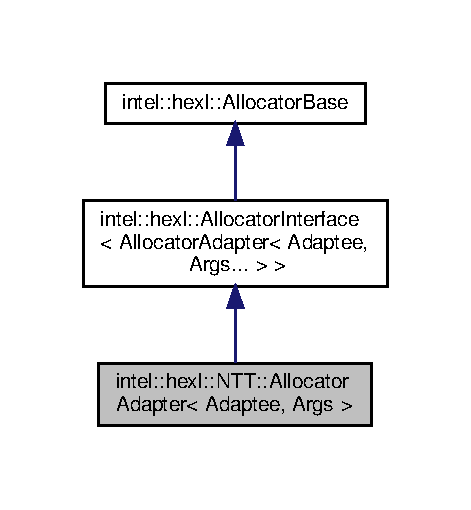
\includegraphics[width=226pt]{structintel_1_1hexl_1_1NTT_1_1AllocatorAdapter__inherit__graph}
\end{center}
\end{figure}


Collaboration diagram for intel\+:\+:hexl\+:\+:N\+TT\+:\+:Allocator\+Adapter$<$ Adaptee, Args $>$\+:
\nopagebreak
\begin{figure}[H]
\begin{center}
\leavevmode
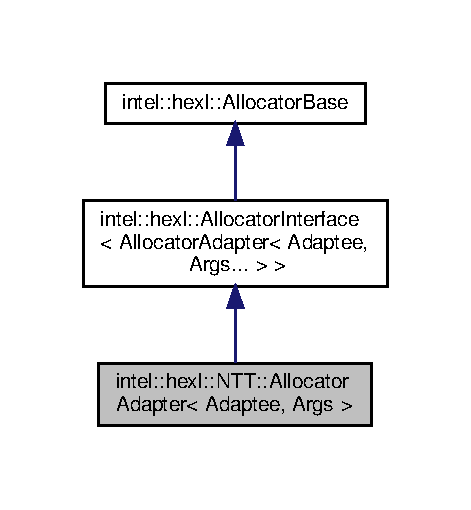
\includegraphics[width=226pt]{structintel_1_1hexl_1_1NTT_1_1AllocatorAdapter__coll__graph}
\end{center}
\end{figure}
\subsection*{Public Member Functions}
\begin{DoxyCompactItemize}
\item 
\hyperlink{structintel_1_1hexl_1_1NTT_1_1AllocatorAdapter_a4403f32f5ed5527a13c2bf12c20a68af}{Allocator\+Adapter} (Adaptee \&\&\+\_\+a, Args \&\&... args)
\item 
\hyperlink{structintel_1_1hexl_1_1NTT_1_1AllocatorAdapter_aee97fbd36cf2299db87f6dbe75f12396}{Allocator\+Adapter} (const Adaptee \&\+\_\+a, Args \&... args)
\item 
void $\ast$ \hyperlink{structintel_1_1hexl_1_1NTT_1_1AllocatorAdapter_a408a6a4b42aef1db5ab7e9b5c8ec2670}{allocate\+\_\+impl} (size\+\_\+t bytes\+\_\+count)
\item 
void \hyperlink{structintel_1_1hexl_1_1NTT_1_1AllocatorAdapter_a123aa02665ce9f2b219ca9b88164e114}{deallocate\+\_\+impl} (void $\ast$p, size\+\_\+t n)
\end{DoxyCompactItemize}


\subsection{Constructor \& Destructor Documentation}
\mbox{\Hypertarget{structintel_1_1hexl_1_1NTT_1_1AllocatorAdapter_a4403f32f5ed5527a13c2bf12c20a68af}\label{structintel_1_1hexl_1_1NTT_1_1AllocatorAdapter_a4403f32f5ed5527a13c2bf12c20a68af}} 
\index{intel\+::hexl\+::\+N\+T\+T\+::\+Allocator\+Adapter@{intel\+::hexl\+::\+N\+T\+T\+::\+Allocator\+Adapter}!Allocator\+Adapter@{Allocator\+Adapter}}
\index{Allocator\+Adapter@{Allocator\+Adapter}!intel\+::hexl\+::\+N\+T\+T\+::\+Allocator\+Adapter@{intel\+::hexl\+::\+N\+T\+T\+::\+Allocator\+Adapter}}
\subsubsection{\texorpdfstring{Allocator\+Adapter()}{AllocatorAdapter()}\hspace{0.1cm}{\footnotesize\ttfamily [1/2]}}
{\footnotesize\ttfamily template$<$class Adaptee , class... Args$>$ \\
\hyperlink{structintel_1_1hexl_1_1NTT_1_1AllocatorAdapter}{intel\+::hexl\+::\+N\+T\+T\+::\+Allocator\+Adapter}$<$ Adaptee, Args $>$\+::\hyperlink{structintel_1_1hexl_1_1NTT_1_1AllocatorAdapter}{Allocator\+Adapter} (\begin{DoxyParamCaption}\item[{Adaptee \&\&}]{\+\_\+a,  }\item[{Args \&\&...}]{args }\end{DoxyParamCaption})\hspace{0.3cm}{\ttfamily [explicit]}}

\mbox{\Hypertarget{structintel_1_1hexl_1_1NTT_1_1AllocatorAdapter_aee97fbd36cf2299db87f6dbe75f12396}\label{structintel_1_1hexl_1_1NTT_1_1AllocatorAdapter_aee97fbd36cf2299db87f6dbe75f12396}} 
\index{intel\+::hexl\+::\+N\+T\+T\+::\+Allocator\+Adapter@{intel\+::hexl\+::\+N\+T\+T\+::\+Allocator\+Adapter}!Allocator\+Adapter@{Allocator\+Adapter}}
\index{Allocator\+Adapter@{Allocator\+Adapter}!intel\+::hexl\+::\+N\+T\+T\+::\+Allocator\+Adapter@{intel\+::hexl\+::\+N\+T\+T\+::\+Allocator\+Adapter}}
\subsubsection{\texorpdfstring{Allocator\+Adapter()}{AllocatorAdapter()}\hspace{0.1cm}{\footnotesize\ttfamily [2/2]}}
{\footnotesize\ttfamily template$<$class Adaptee , class... Args$>$ \\
\hyperlink{structintel_1_1hexl_1_1NTT_1_1AllocatorAdapter}{intel\+::hexl\+::\+N\+T\+T\+::\+Allocator\+Adapter}$<$ Adaptee, Args $>$\+::\hyperlink{structintel_1_1hexl_1_1NTT_1_1AllocatorAdapter}{Allocator\+Adapter} (\begin{DoxyParamCaption}\item[{const Adaptee \&}]{\+\_\+a,  }\item[{Args \&...}]{args }\end{DoxyParamCaption})}



\subsection{Member Function Documentation}
\mbox{\Hypertarget{structintel_1_1hexl_1_1NTT_1_1AllocatorAdapter_a408a6a4b42aef1db5ab7e9b5c8ec2670}\label{structintel_1_1hexl_1_1NTT_1_1AllocatorAdapter_a408a6a4b42aef1db5ab7e9b5c8ec2670}} 
\index{intel\+::hexl\+::\+N\+T\+T\+::\+Allocator\+Adapter@{intel\+::hexl\+::\+N\+T\+T\+::\+Allocator\+Adapter}!allocate\+\_\+impl@{allocate\+\_\+impl}}
\index{allocate\+\_\+impl@{allocate\+\_\+impl}!intel\+::hexl\+::\+N\+T\+T\+::\+Allocator\+Adapter@{intel\+::hexl\+::\+N\+T\+T\+::\+Allocator\+Adapter}}
\subsubsection{\texorpdfstring{allocate\+\_\+impl()}{allocate\_impl()}}
{\footnotesize\ttfamily template$<$class Adaptee , class... Args$>$ \\
void$\ast$ \hyperlink{structintel_1_1hexl_1_1NTT_1_1AllocatorAdapter}{intel\+::hexl\+::\+N\+T\+T\+::\+Allocator\+Adapter}$<$ Adaptee, Args $>$\+::allocate\+\_\+impl (\begin{DoxyParamCaption}\item[{size\+\_\+t}]{bytes\+\_\+count }\end{DoxyParamCaption})}

\mbox{\Hypertarget{structintel_1_1hexl_1_1NTT_1_1AllocatorAdapter_a123aa02665ce9f2b219ca9b88164e114}\label{structintel_1_1hexl_1_1NTT_1_1AllocatorAdapter_a123aa02665ce9f2b219ca9b88164e114}} 
\index{intel\+::hexl\+::\+N\+T\+T\+::\+Allocator\+Adapter@{intel\+::hexl\+::\+N\+T\+T\+::\+Allocator\+Adapter}!deallocate\+\_\+impl@{deallocate\+\_\+impl}}
\index{deallocate\+\_\+impl@{deallocate\+\_\+impl}!intel\+::hexl\+::\+N\+T\+T\+::\+Allocator\+Adapter@{intel\+::hexl\+::\+N\+T\+T\+::\+Allocator\+Adapter}}
\subsubsection{\texorpdfstring{deallocate\+\_\+impl()}{deallocate\_impl()}}
{\footnotesize\ttfamily template$<$class Adaptee , class... Args$>$ \\
void \hyperlink{structintel_1_1hexl_1_1NTT_1_1AllocatorAdapter}{intel\+::hexl\+::\+N\+T\+T\+::\+Allocator\+Adapter}$<$ Adaptee, Args $>$\+::deallocate\+\_\+impl (\begin{DoxyParamCaption}\item[{void $\ast$}]{p,  }\item[{size\+\_\+t}]{n }\end{DoxyParamCaption})}



The documentation for this struct was generated from the following file\+:\begin{DoxyCompactItemize}
\item 
\hyperlink{ntt_8hpp}{ntt.\+hpp}\end{DoxyCompactItemize}

\hypertarget{structintel_1_1hexl_1_1AllocatorBase}{}\section{intel\+:\+:hexl\+:\+:Allocator\+Base Struct Reference}
\label{structintel_1_1hexl_1_1AllocatorBase}\index{intel\+::hexl\+::\+Allocator\+Base@{intel\+::hexl\+::\+Allocator\+Base}}


{\ttfamily \#include $<$allocator.\+hpp$>$}



Inheritance diagram for intel\+:\+:hexl\+:\+:Allocator\+Base\+:
\nopagebreak
\begin{figure}[H]
\begin{center}
\leavevmode
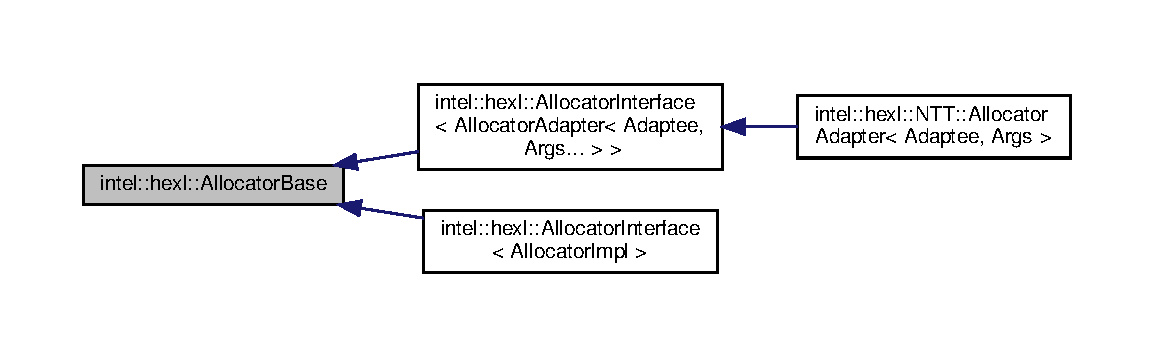
\includegraphics[width=350pt]{structintel_1_1hexl_1_1AllocatorBase__inherit__graph}
\end{center}
\end{figure}
\subsection*{Public Member Functions}
\begin{DoxyCompactItemize}
\item 
virtual \hyperlink{structintel_1_1hexl_1_1AllocatorBase_ac8a2afdc70cef8b7c9342aa2281ea4d5}{$\sim$\+Allocator\+Base} () noexcept
\item 
virtual void $\ast$ \hyperlink{structintel_1_1hexl_1_1AllocatorBase_aadf587e7617fbace2e9d3b4f9d9e8af0}{allocate} (size\+\_\+t bytes\+\_\+count)=0
\item 
virtual void \hyperlink{structintel_1_1hexl_1_1AllocatorBase_a0f03686f9b78728d4d228ceaf4c2948e}{deallocate} (void $\ast$p, size\+\_\+t n)=0
\end{DoxyCompactItemize}


\subsection{Constructor \& Destructor Documentation}
\mbox{\Hypertarget{structintel_1_1hexl_1_1AllocatorBase_ac8a2afdc70cef8b7c9342aa2281ea4d5}\label{structintel_1_1hexl_1_1AllocatorBase_ac8a2afdc70cef8b7c9342aa2281ea4d5}} 
\index{intel\+::hexl\+::\+Allocator\+Base@{intel\+::hexl\+::\+Allocator\+Base}!````~Allocator\+Base@{$\sim$\+Allocator\+Base}}
\index{````~Allocator\+Base@{$\sim$\+Allocator\+Base}!intel\+::hexl\+::\+Allocator\+Base@{intel\+::hexl\+::\+Allocator\+Base}}
\subsubsection{\texorpdfstring{$\sim$\+Allocator\+Base()}{~AllocatorBase()}}
{\footnotesize\ttfamily virtual intel\+::hexl\+::\+Allocator\+Base\+::$\sim$\+Allocator\+Base (\begin{DoxyParamCaption}{ }\end{DoxyParamCaption})\hspace{0.3cm}{\ttfamily [inline]}, {\ttfamily [virtual]}, {\ttfamily [noexcept]}}



\subsection{Member Function Documentation}
\mbox{\Hypertarget{structintel_1_1hexl_1_1AllocatorBase_aadf587e7617fbace2e9d3b4f9d9e8af0}\label{structintel_1_1hexl_1_1AllocatorBase_aadf587e7617fbace2e9d3b4f9d9e8af0}} 
\index{intel\+::hexl\+::\+Allocator\+Base@{intel\+::hexl\+::\+Allocator\+Base}!allocate@{allocate}}
\index{allocate@{allocate}!intel\+::hexl\+::\+Allocator\+Base@{intel\+::hexl\+::\+Allocator\+Base}}
\subsubsection{\texorpdfstring{allocate()}{allocate()}}
{\footnotesize\ttfamily virtual void$\ast$ intel\+::hexl\+::\+Allocator\+Base\+::allocate (\begin{DoxyParamCaption}\item[{size\+\_\+t}]{bytes\+\_\+count }\end{DoxyParamCaption})\hspace{0.3cm}{\ttfamily [pure virtual]}}



Implemented in \hyperlink{structintel_1_1hexl_1_1AllocatorInterface_a02d2d7918ea916fce443ba2f5dbaa8d1}{intel\+::hexl\+::\+Allocator\+Interface$<$ Allocator\+Impl $>$}, and \hyperlink{structintel_1_1hexl_1_1AllocatorInterface_a02d2d7918ea916fce443ba2f5dbaa8d1}{intel\+::hexl\+::\+Allocator\+Interface$<$ Allocator\+Adapter$<$ Adaptee, Args... $>$ $>$}.

\mbox{\Hypertarget{structintel_1_1hexl_1_1AllocatorBase_a0f03686f9b78728d4d228ceaf4c2948e}\label{structintel_1_1hexl_1_1AllocatorBase_a0f03686f9b78728d4d228ceaf4c2948e}} 
\index{intel\+::hexl\+::\+Allocator\+Base@{intel\+::hexl\+::\+Allocator\+Base}!deallocate@{deallocate}}
\index{deallocate@{deallocate}!intel\+::hexl\+::\+Allocator\+Base@{intel\+::hexl\+::\+Allocator\+Base}}
\subsubsection{\texorpdfstring{deallocate()}{deallocate()}}
{\footnotesize\ttfamily virtual void intel\+::hexl\+::\+Allocator\+Base\+::deallocate (\begin{DoxyParamCaption}\item[{void $\ast$}]{p,  }\item[{size\+\_\+t}]{n }\end{DoxyParamCaption})\hspace{0.3cm}{\ttfamily [pure virtual]}}



Implemented in \hyperlink{structintel_1_1hexl_1_1AllocatorInterface_a2684feec3b8f3cfba626b46912b4cec5}{intel\+::hexl\+::\+Allocator\+Interface$<$ Allocator\+Impl $>$}, and \hyperlink{structintel_1_1hexl_1_1AllocatorInterface_a2684feec3b8f3cfba626b46912b4cec5}{intel\+::hexl\+::\+Allocator\+Interface$<$ Allocator\+Adapter$<$ Adaptee, Args... $>$ $>$}.



The documentation for this struct was generated from the following file\+:\begin{DoxyCompactItemize}
\item 
\hyperlink{allocator_8hpp}{allocator.\+hpp}\end{DoxyCompactItemize}

\hypertarget{structintel_1_1hexl_1_1AllocatorInterface}{}\section{intel\+:\+:hexl\+:\+:Allocator\+Interface$<$ Allocator\+Impl $>$ Struct Template Reference}
\label{structintel_1_1hexl_1_1AllocatorInterface}\index{intel\+::hexl\+::\+Allocator\+Interface$<$ Allocator\+Impl $>$@{intel\+::hexl\+::\+Allocator\+Interface$<$ Allocator\+Impl $>$}}


{\ttfamily \#include $<$allocator.\+hpp$>$}



Inheritance diagram for intel\+:\+:hexl\+:\+:Allocator\+Interface$<$ Allocator\+Impl $>$\+:
\nopagebreak
\begin{figure}[H]
\begin{center}
\leavevmode
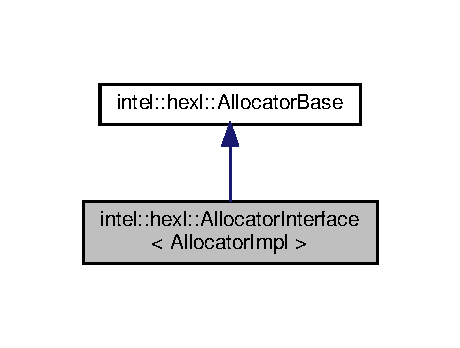
\includegraphics[width=221pt]{structintel_1_1hexl_1_1AllocatorInterface__inherit__graph}
\end{center}
\end{figure}


Collaboration diagram for intel\+:\+:hexl\+:\+:Allocator\+Interface$<$ Allocator\+Impl $>$\+:
\nopagebreak
\begin{figure}[H]
\begin{center}
\leavevmode
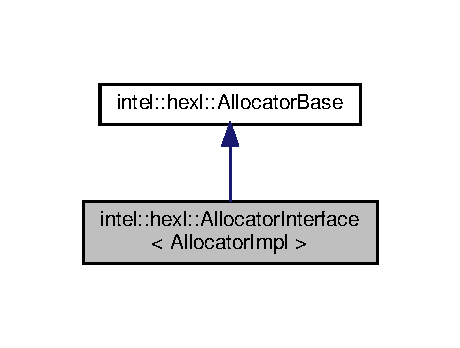
\includegraphics[width=221pt]{structintel_1_1hexl_1_1AllocatorInterface__coll__graph}
\end{center}
\end{figure}
\subsection*{Public Member Functions}
\begin{DoxyCompactItemize}
\item 
void $\ast$ \hyperlink{structintel_1_1hexl_1_1AllocatorInterface_a02d2d7918ea916fce443ba2f5dbaa8d1}{allocate} (size\+\_\+t bytes\+\_\+count) override
\item 
void \hyperlink{structintel_1_1hexl_1_1AllocatorInterface_a2684feec3b8f3cfba626b46912b4cec5}{deallocate} (void $\ast$p, size\+\_\+t n) override
\end{DoxyCompactItemize}


\subsection{Member Function Documentation}
\mbox{\Hypertarget{structintel_1_1hexl_1_1AllocatorInterface_a02d2d7918ea916fce443ba2f5dbaa8d1}\label{structintel_1_1hexl_1_1AllocatorInterface_a02d2d7918ea916fce443ba2f5dbaa8d1}} 
\index{intel\+::hexl\+::\+Allocator\+Interface@{intel\+::hexl\+::\+Allocator\+Interface}!allocate@{allocate}}
\index{allocate@{allocate}!intel\+::hexl\+::\+Allocator\+Interface@{intel\+::hexl\+::\+Allocator\+Interface}}
\subsubsection{\texorpdfstring{allocate()}{allocate()}}
{\footnotesize\ttfamily template$<$class Allocator\+Impl$>$ \\
void$\ast$ \hyperlink{structintel_1_1hexl_1_1AllocatorInterface}{intel\+::hexl\+::\+Allocator\+Interface}$<$ Allocator\+Impl $>$\+::allocate (\begin{DoxyParamCaption}\item[{size\+\_\+t}]{bytes\+\_\+count }\end{DoxyParamCaption})\hspace{0.3cm}{\ttfamily [inline]}, {\ttfamily [override]}, {\ttfamily [virtual]}}



Implements \hyperlink{structintel_1_1hexl_1_1AllocatorBase_aadf587e7617fbace2e9d3b4f9d9e8af0}{intel\+::hexl\+::\+Allocator\+Base}.

\mbox{\Hypertarget{structintel_1_1hexl_1_1AllocatorInterface_a2684feec3b8f3cfba626b46912b4cec5}\label{structintel_1_1hexl_1_1AllocatorInterface_a2684feec3b8f3cfba626b46912b4cec5}} 
\index{intel\+::hexl\+::\+Allocator\+Interface@{intel\+::hexl\+::\+Allocator\+Interface}!deallocate@{deallocate}}
\index{deallocate@{deallocate}!intel\+::hexl\+::\+Allocator\+Interface@{intel\+::hexl\+::\+Allocator\+Interface}}
\subsubsection{\texorpdfstring{deallocate()}{deallocate()}}
{\footnotesize\ttfamily template$<$class Allocator\+Impl$>$ \\
void \hyperlink{structintel_1_1hexl_1_1AllocatorInterface}{intel\+::hexl\+::\+Allocator\+Interface}$<$ Allocator\+Impl $>$\+::deallocate (\begin{DoxyParamCaption}\item[{void $\ast$}]{p,  }\item[{size\+\_\+t}]{n }\end{DoxyParamCaption})\hspace{0.3cm}{\ttfamily [inline]}, {\ttfamily [override]}, {\ttfamily [virtual]}}



Implements \hyperlink{structintel_1_1hexl_1_1AllocatorBase_a0f03686f9b78728d4d228ceaf4c2948e}{intel\+::hexl\+::\+Allocator\+Base}.



The documentation for this struct was generated from the following file\+:\begin{DoxyCompactItemize}
\item 
\hyperlink{allocator_8hpp}{allocator.\+hpp}\end{DoxyCompactItemize}

\hypertarget{classintel_1_1hexl_1_1NTT}{}\section{intel\+:\+:hexl\+:\+:N\+TT Class Reference}
\label{classintel_1_1hexl_1_1NTT}\index{intel\+::hexl\+::\+N\+TT@{intel\+::hexl\+::\+N\+TT}}


Performs negacyclic forward and inverse number-\/theoretic transform (\hyperlink{classintel_1_1hexl_1_1NTT}{N\+TT}), commonly used in R\+L\+WE cryptography.  




{\ttfamily \#include $<$ntt.\+hpp$>$}

\subsection*{Classes}
\begin{DoxyCompactItemize}
\item 
struct \hyperlink{structintel_1_1hexl_1_1NTT_1_1AllocatorAdapter}{Allocator\+Adapter}
\end{DoxyCompactItemize}
\subsection*{Public Member Functions}
\begin{DoxyCompactItemize}
\item 
\hyperlink{classintel_1_1hexl_1_1NTT_ade0447617b50232d2a076f99e672d15c}{N\+TT} ()
\begin{DoxyCompactList}\small\item\em Initializes an empty \hyperlink{classintel_1_1hexl_1_1NTT}{N\+TT} object. \end{DoxyCompactList}\item 
\hyperlink{classintel_1_1hexl_1_1NTT_ab6fca1753db0834c692232e8897c725f}{$\sim$\+N\+TT} ()
\begin{DoxyCompactList}\small\item\em Destructs the \hyperlink{classintel_1_1hexl_1_1NTT}{N\+TT} object. \end{DoxyCompactList}\item 
\hyperlink{classintel_1_1hexl_1_1NTT_a7a86355beefbe191d0e77618eeaaf6b7}{N\+TT} (uint64\+\_\+t degree, uint64\+\_\+t q, std\+::shared\+\_\+ptr$<$ \hyperlink{structintel_1_1hexl_1_1AllocatorBase}{Allocator\+Base} $>$ alloc\+\_\+ptr=\{\})
\begin{DoxyCompactList}\small\item\em Performs pre-\/computation necessary for forward and inverse transforms. \end{DoxyCompactList}\item 
{\footnotesize template$<$class Allocator , class... Allocator\+Args$>$ }\\\hyperlink{classintel_1_1hexl_1_1NTT_a716fd07255e9b68fec80e2a9b98841f4}{N\+TT} (uint64\+\_\+t degree, uint64\+\_\+t q, Allocator \&\&a, Allocator\+Args \&\&... args)
\item 
\hyperlink{classintel_1_1hexl_1_1NTT_ac5ef577bf39789c1e200b7d5a7b65989}{N\+TT} (uint64\+\_\+t degree, uint64\+\_\+t q, uint64\+\_\+t root\+\_\+of\+\_\+unity, std\+::shared\+\_\+ptr$<$ \hyperlink{structintel_1_1hexl_1_1AllocatorBase}{Allocator\+Base} $>$ alloc\+\_\+ptr=\{\})
\begin{DoxyCompactList}\small\item\em Initializes an \hyperlink{classintel_1_1hexl_1_1NTT}{N\+TT} object with degree {\ttfamily degree} and modulus {\ttfamily q}. \end{DoxyCompactList}\item 
{\footnotesize template$<$class Allocator , class... Allocator\+Args$>$ }\\\hyperlink{classintel_1_1hexl_1_1NTT_a831df901cf9ea5a83e5d628cdbd36671}{N\+TT} (uint64\+\_\+t degree, uint64\+\_\+t q, uint64\+\_\+t root\+\_\+of\+\_\+unity, Allocator \&\&a, Allocator\+Args \&\&... args)
\item 
void \hyperlink{classintel_1_1hexl_1_1NTT_a7f8dac5ff3fc117d3e7259762a716140}{Compute\+Forward} (uint64\+\_\+t $\ast$result, const uint64\+\_\+t $\ast$operand, uint64\+\_\+t input\+\_\+mod\+\_\+factor, uint64\+\_\+t output\+\_\+mod\+\_\+factor)
\begin{DoxyCompactList}\small\item\em Compute forward \hyperlink{classintel_1_1hexl_1_1NTT}{N\+TT}. Results are bit-\/reversed. \end{DoxyCompactList}\item 
void \hyperlink{classintel_1_1hexl_1_1NTT_a31e78375dcafd5df85cb1259a9156a9a}{Compute\+Inverse} (uint64\+\_\+t $\ast$result, const uint64\+\_\+t $\ast$operand, uint64\+\_\+t input\+\_\+mod\+\_\+factor, uint64\+\_\+t output\+\_\+mod\+\_\+factor)
\end{DoxyCompactItemize}


\subsection{Detailed Description}
Performs negacyclic forward and inverse number-\/theoretic transform (\hyperlink{classintel_1_1hexl_1_1NTT}{N\+TT}), commonly used in R\+L\+WE cryptography. 

The number-\/theoretic transform (\hyperlink{classintel_1_1hexl_1_1NTT}{N\+TT}) specializes the discrete Fourier transform (D\+FT) to the finite field $ \mathbb{Z}_q[X] / (X^N + 1) $. 

\subsection{Constructor \& Destructor Documentation}
\mbox{\Hypertarget{classintel_1_1hexl_1_1NTT_ade0447617b50232d2a076f99e672d15c}\label{classintel_1_1hexl_1_1NTT_ade0447617b50232d2a076f99e672d15c}} 
\index{intel\+::hexl\+::\+N\+TT@{intel\+::hexl\+::\+N\+TT}!N\+TT@{N\+TT}}
\index{N\+TT@{N\+TT}!intel\+::hexl\+::\+N\+TT@{intel\+::hexl\+::\+N\+TT}}
\subsubsection{\texorpdfstring{N\+T\+T()}{NTT()}\hspace{0.1cm}{\footnotesize\ttfamily [1/5]}}
{\footnotesize\ttfamily intel\+::hexl\+::\+N\+T\+T\+::\+N\+TT (\begin{DoxyParamCaption}{ }\end{DoxyParamCaption})}



Initializes an empty \hyperlink{classintel_1_1hexl_1_1NTT}{N\+TT} object. 

\mbox{\Hypertarget{classintel_1_1hexl_1_1NTT_ab6fca1753db0834c692232e8897c725f}\label{classintel_1_1hexl_1_1NTT_ab6fca1753db0834c692232e8897c725f}} 
\index{intel\+::hexl\+::\+N\+TT@{intel\+::hexl\+::\+N\+TT}!````~N\+TT@{$\sim$\+N\+TT}}
\index{````~N\+TT@{$\sim$\+N\+TT}!intel\+::hexl\+::\+N\+TT@{intel\+::hexl\+::\+N\+TT}}
\subsubsection{\texorpdfstring{$\sim$\+N\+T\+T()}{~NTT()}}
{\footnotesize\ttfamily intel\+::hexl\+::\+N\+T\+T\+::$\sim$\+N\+TT (\begin{DoxyParamCaption}{ }\end{DoxyParamCaption})}



Destructs the \hyperlink{classintel_1_1hexl_1_1NTT}{N\+TT} object. 

\mbox{\Hypertarget{classintel_1_1hexl_1_1NTT_a7a86355beefbe191d0e77618eeaaf6b7}\label{classintel_1_1hexl_1_1NTT_a7a86355beefbe191d0e77618eeaaf6b7}} 
\index{intel\+::hexl\+::\+N\+TT@{intel\+::hexl\+::\+N\+TT}!N\+TT@{N\+TT}}
\index{N\+TT@{N\+TT}!intel\+::hexl\+::\+N\+TT@{intel\+::hexl\+::\+N\+TT}}
\subsubsection{\texorpdfstring{N\+T\+T()}{NTT()}\hspace{0.1cm}{\footnotesize\ttfamily [2/5]}}
{\footnotesize\ttfamily intel\+::hexl\+::\+N\+T\+T\+::\+N\+TT (\begin{DoxyParamCaption}\item[{uint64\+\_\+t}]{degree,  }\item[{uint64\+\_\+t}]{q,  }\item[{std\+::shared\+\_\+ptr$<$ \hyperlink{structintel_1_1hexl_1_1AllocatorBase}{Allocator\+Base} $>$}]{alloc\+\_\+ptr = {\ttfamily \{\}} }\end{DoxyParamCaption})}



Performs pre-\/computation necessary for forward and inverse transforms. 

Initializes an \hyperlink{classintel_1_1hexl_1_1NTT}{N\+TT} object with degree {\ttfamily degree} and modulus {\ttfamily q}. 
\begin{DoxyParams}[1]{Parameters}
\mbox{\tt in}  & {\em degree} & also known as N. Size of the \hyperlink{classintel_1_1hexl_1_1NTT}{N\+TT} transform. Must be a power of 2 \\
\hline
\mbox{\tt in}  & {\em q} & Prime modulus. Must satisfy $ q == 1 \mod 2N $ \\
\hline
\mbox{\tt in}  & {\em alloc\+\_\+ptr} & Custom memory allocator used for intermediate calculations \\
\hline
\end{DoxyParams}
\mbox{\Hypertarget{classintel_1_1hexl_1_1NTT_a716fd07255e9b68fec80e2a9b98841f4}\label{classintel_1_1hexl_1_1NTT_a716fd07255e9b68fec80e2a9b98841f4}} 
\index{intel\+::hexl\+::\+N\+TT@{intel\+::hexl\+::\+N\+TT}!N\+TT@{N\+TT}}
\index{N\+TT@{N\+TT}!intel\+::hexl\+::\+N\+TT@{intel\+::hexl\+::\+N\+TT}}
\subsubsection{\texorpdfstring{N\+T\+T()}{NTT()}\hspace{0.1cm}{\footnotesize\ttfamily [3/5]}}
{\footnotesize\ttfamily template$<$class Allocator , class... Allocator\+Args$>$ \\
intel\+::hexl\+::\+N\+T\+T\+::\+N\+TT (\begin{DoxyParamCaption}\item[{uint64\+\_\+t}]{degree,  }\item[{uint64\+\_\+t}]{q,  }\item[{Allocator \&\&}]{a,  }\item[{Allocator\+Args \&\&...}]{args }\end{DoxyParamCaption})\hspace{0.3cm}{\ttfamily [inline]}}

\mbox{\Hypertarget{classintel_1_1hexl_1_1NTT_ac5ef577bf39789c1e200b7d5a7b65989}\label{classintel_1_1hexl_1_1NTT_ac5ef577bf39789c1e200b7d5a7b65989}} 
\index{intel\+::hexl\+::\+N\+TT@{intel\+::hexl\+::\+N\+TT}!N\+TT@{N\+TT}}
\index{N\+TT@{N\+TT}!intel\+::hexl\+::\+N\+TT@{intel\+::hexl\+::\+N\+TT}}
\subsubsection{\texorpdfstring{N\+T\+T()}{NTT()}\hspace{0.1cm}{\footnotesize\ttfamily [4/5]}}
{\footnotesize\ttfamily intel\+::hexl\+::\+N\+T\+T\+::\+N\+TT (\begin{DoxyParamCaption}\item[{uint64\+\_\+t}]{degree,  }\item[{uint64\+\_\+t}]{q,  }\item[{uint64\+\_\+t}]{root\+\_\+of\+\_\+unity,  }\item[{std\+::shared\+\_\+ptr$<$ \hyperlink{structintel_1_1hexl_1_1AllocatorBase}{Allocator\+Base} $>$}]{alloc\+\_\+ptr = {\ttfamily \{\}} }\end{DoxyParamCaption})}



Initializes an \hyperlink{classintel_1_1hexl_1_1NTT}{N\+TT} object with degree {\ttfamily degree} and modulus {\ttfamily q}. 


\begin{DoxyParams}[1]{Parameters}
\mbox{\tt in}  & {\em degree} & also known as N. Size of the \hyperlink{classintel_1_1hexl_1_1NTT}{N\+TT} transform. Must be a power of 2 \\
\hline
\mbox{\tt in}  & {\em q} & Prime modulus. Must satisfy $ q == 1 \mod 2N $ \\
\hline
\mbox{\tt in}  & {\em root\+\_\+of\+\_\+unity} & 2N\textquotesingle{}th root of unity in $ \mathbb{Z_q} $. \\
\hline
\mbox{\tt in}  & {\em alloc\+\_\+ptr} & Custom memory allocator used for intermediate calculations\\
\hline
\end{DoxyParams}
Performs pre-\/computation necessary for forward and inverse transforms \mbox{\Hypertarget{classintel_1_1hexl_1_1NTT_a831df901cf9ea5a83e5d628cdbd36671}\label{classintel_1_1hexl_1_1NTT_a831df901cf9ea5a83e5d628cdbd36671}} 
\index{intel\+::hexl\+::\+N\+TT@{intel\+::hexl\+::\+N\+TT}!N\+TT@{N\+TT}}
\index{N\+TT@{N\+TT}!intel\+::hexl\+::\+N\+TT@{intel\+::hexl\+::\+N\+TT}}
\subsubsection{\texorpdfstring{N\+T\+T()}{NTT()}\hspace{0.1cm}{\footnotesize\ttfamily [5/5]}}
{\footnotesize\ttfamily template$<$class Allocator , class... Allocator\+Args$>$ \\
intel\+::hexl\+::\+N\+T\+T\+::\+N\+TT (\begin{DoxyParamCaption}\item[{uint64\+\_\+t}]{degree,  }\item[{uint64\+\_\+t}]{q,  }\item[{uint64\+\_\+t}]{root\+\_\+of\+\_\+unity,  }\item[{Allocator \&\&}]{a,  }\item[{Allocator\+Args \&\&...}]{args }\end{DoxyParamCaption})\hspace{0.3cm}{\ttfamily [inline]}}



\subsection{Member Function Documentation}
\mbox{\Hypertarget{classintel_1_1hexl_1_1NTT_a7f8dac5ff3fc117d3e7259762a716140}\label{classintel_1_1hexl_1_1NTT_a7f8dac5ff3fc117d3e7259762a716140}} 
\index{intel\+::hexl\+::\+N\+TT@{intel\+::hexl\+::\+N\+TT}!Compute\+Forward@{Compute\+Forward}}
\index{Compute\+Forward@{Compute\+Forward}!intel\+::hexl\+::\+N\+TT@{intel\+::hexl\+::\+N\+TT}}
\subsubsection{\texorpdfstring{Compute\+Forward()}{ComputeForward()}}
{\footnotesize\ttfamily void intel\+::hexl\+::\+N\+T\+T\+::\+Compute\+Forward (\begin{DoxyParamCaption}\item[{uint64\+\_\+t $\ast$}]{result,  }\item[{const uint64\+\_\+t $\ast$}]{operand,  }\item[{uint64\+\_\+t}]{input\+\_\+mod\+\_\+factor,  }\item[{uint64\+\_\+t}]{output\+\_\+mod\+\_\+factor }\end{DoxyParamCaption})}



Compute forward \hyperlink{classintel_1_1hexl_1_1NTT}{N\+TT}. Results are bit-\/reversed. 


\begin{DoxyParams}[1]{Parameters}
\mbox{\tt out}  & {\em result} & Stores the result \\
\hline
\mbox{\tt in}  & {\em operand} & Data on which to compute the \hyperlink{classintel_1_1hexl_1_1NTT}{N\+TT} \\
\hline
\mbox{\tt in}  & {\em input\+\_\+mod\+\_\+factor} & Assume input {\ttfamily operand} are in \mbox{[}0, input\+\_\+mod\+\_\+factor $\ast$ q). Must be 1, 2 or 4. \\
\hline
\mbox{\tt in}  & {\em output\+\_\+mod\+\_\+factor} & Returns output {\ttfamily operand} in \mbox{[}0, output\+\_\+mod\+\_\+factor $\ast$ q). Must be 1 or 4. \\
\hline
\end{DoxyParams}
\mbox{\Hypertarget{classintel_1_1hexl_1_1NTT_a31e78375dcafd5df85cb1259a9156a9a}\label{classintel_1_1hexl_1_1NTT_a31e78375dcafd5df85cb1259a9156a9a}} 
\index{intel\+::hexl\+::\+N\+TT@{intel\+::hexl\+::\+N\+TT}!Compute\+Inverse@{Compute\+Inverse}}
\index{Compute\+Inverse@{Compute\+Inverse}!intel\+::hexl\+::\+N\+TT@{intel\+::hexl\+::\+N\+TT}}
\subsubsection{\texorpdfstring{Compute\+Inverse()}{ComputeInverse()}}
{\footnotesize\ttfamily void intel\+::hexl\+::\+N\+T\+T\+::\+Compute\+Inverse (\begin{DoxyParamCaption}\item[{uint64\+\_\+t $\ast$}]{result,  }\item[{const uint64\+\_\+t $\ast$}]{operand,  }\item[{uint64\+\_\+t}]{input\+\_\+mod\+\_\+factor,  }\item[{uint64\+\_\+t}]{output\+\_\+mod\+\_\+factor }\end{DoxyParamCaption})}

Compute inverse \hyperlink{classintel_1_1hexl_1_1NTT}{N\+TT}. Results are bit-\/reversed. 
\begin{DoxyParams}[1]{Parameters}
\mbox{\tt out}  & {\em result} & Stores the result \\
\hline
\mbox{\tt in}  & {\em operand} & Data on which to compute the \hyperlink{classintel_1_1hexl_1_1NTT}{N\+TT} \\
\hline
\mbox{\tt in}  & {\em input\+\_\+mod\+\_\+factor} & Assume input {\ttfamily operand} are in \mbox{[}0, input\+\_\+mod\+\_\+factor $\ast$ q). Must be 1 or 2. \\
\hline
\mbox{\tt in}  & {\em output\+\_\+mod\+\_\+factor} & Returns output {\ttfamily operand} in \mbox{[}0, output\+\_\+mod\+\_\+factor $\ast$ q). Must be 1 or 2. \\
\hline
\end{DoxyParams}


The documentation for this class was generated from the following file\+:\begin{DoxyCompactItemize}
\item 
\hyperlink{ntt_8hpp}{ntt.\+hpp}\end{DoxyCompactItemize}

\chapter{File Documentation}
\hypertarget{allocator_8hpp}{}\section{allocator.\+hpp File Reference}
\label{allocator_8hpp}\index{allocator.\+hpp@{allocator.\+hpp}}
{\ttfamily \#include $<$cstddef$>$}\newline
Include dependency graph for allocator.\+hpp\+:
\nopagebreak
\begin{figure}[H]
\begin{center}
\leavevmode
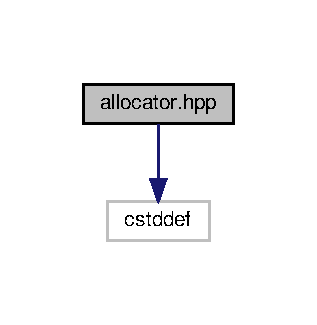
\includegraphics[width=152pt]{allocator_8hpp__incl}
\end{center}
\end{figure}
This graph shows which files directly or indirectly include this file\+:
\nopagebreak
\begin{figure}[H]
\begin{center}
\leavevmode
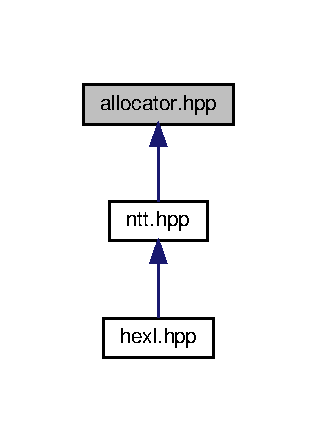
\includegraphics[width=152pt]{allocator_8hpp__dep__incl}
\end{center}
\end{figure}
\subsection*{Classes}
\begin{DoxyCompactItemize}
\item 
struct \hyperlink{structintel_1_1hexl_1_1AllocatorBase}{intel\+::hexl\+::\+Allocator\+Base}
\item 
struct \hyperlink{structintel_1_1hexl_1_1AllocatorInterface}{intel\+::hexl\+::\+Allocator\+Interface$<$ Allocator\+Impl $>$}
\end{DoxyCompactItemize}
\subsection*{Namespaces}
\begin{DoxyCompactItemize}
\item 
 \hyperlink{namespaceintel}{intel}
\item 
 \hyperlink{namespaceintel_1_1hexl}{intel\+::hexl}
\end{DoxyCompactItemize}

\hypertarget{eltwise-add-mod_8hpp}{}\doxysection{eltwise-\/add-\/mod.hpp File Reference}
\label{eltwise-add-mod_8hpp}\index{eltwise-\/add-\/mod.hpp@{eltwise-\/add-\/mod.hpp}}
{\ttfamily \#include $<$stdint.\+h$>$}\newline
\doxysubsection*{Namespaces}
\begin{DoxyCompactItemize}
\item 
namespace \mbox{\hyperlink{namespaceintel}{intel}}
\item 
namespace \mbox{\hyperlink{namespaceintel_1_1hexl}{intel\+::hexl}}
\end{DoxyCompactItemize}
\doxysubsection*{Functions}
\begin{DoxyCompactItemize}
\item 
void \mbox{\hyperlink{namespaceintel_1_1hexl_a319244a133f57825ba7e593ad5c71709}{intel\+::hexl\+::\+Eltwise\+Add\+Mod}} (uint64\+\_\+t $\ast$result, const uint64\+\_\+t $\ast$operand1, const uint64\+\_\+t $\ast$operand2, uint64\+\_\+t n, uint64\+\_\+t modulus)
\begin{DoxyCompactList}\small\item\em Adds two vectors elementwise with modular reduction. \end{DoxyCompactList}\end{DoxyCompactItemize}

\hypertarget{eltwise-cmp-add_8hpp}{}\doxysection{/\+Users/fboemer/repos/\+D\+B\+I\+O/intel-\/hexl/hexl/include/hexl/eltwise/eltwise-\/cmp-\/add.hpp File Reference}
\label{eltwise-cmp-add_8hpp}\index{/Users/fboemer/repos/DBIO/intel-\/hexl/hexl/include/hexl/eltwise/eltwise-\/cmp-\/add.hpp@{/Users/fboemer/repos/DBIO/intel-\/hexl/hexl/include/hexl/eltwise/eltwise-\/cmp-\/add.hpp}}
{\ttfamily \#include $<$stdint.\+h$>$}\newline
{\ttfamily \#include \char`\"{}hexl/util/util.\+hpp\char`\"{}}\newline
\doxysubsection*{Namespaces}
\begin{DoxyCompactItemize}
\item 
 \mbox{\hyperlink{namespaceintel}{intel}}
\item 
 \mbox{\hyperlink{namespaceintel_1_1hexl}{intel\+::hexl}}
\end{DoxyCompactItemize}
\doxysubsection*{Functions}
\begin{DoxyCompactItemize}
\item 
void \mbox{\hyperlink{namespaceintel_1_1hexl_a5c4fd2ceb53b94efa5f5a959d7ee9819}{intel\+::hexl\+::\+Eltwise\+Cmp\+Add}} (uint64\+\_\+t $\ast$result, const uint64\+\_\+t $\ast$operand1, uint64\+\_\+t n, C\+M\+P\+I\+NT cmp, uint64\+\_\+t bound, uint64\+\_\+t diff)
\begin{DoxyCompactList}\small\item\em Computes element-\/wise conditional addition. \end{DoxyCompactList}\end{DoxyCompactItemize}

\hypertarget{eltwise-cmp-sub-mod_8hpp}{}\doxysection{eltwise-\/cmp-\/sub-\/mod.hpp File Reference}
\label{eltwise-cmp-sub-mod_8hpp}\index{eltwise-\/cmp-\/sub-\/mod.hpp@{eltwise-\/cmp-\/sub-\/mod.hpp}}
{\ttfamily \#include $<$stdint.\+h$>$}\newline
{\ttfamily \#include \char`\"{}hexl/util/util.\+hpp\char`\"{}}\newline
\doxysubsection*{Namespaces}
\begin{DoxyCompactItemize}
\item 
namespace \mbox{\hyperlink{namespaceintel}{intel}}
\item 
namespace \mbox{\hyperlink{namespaceintel_1_1hexl}{intel\+::hexl}}
\end{DoxyCompactItemize}
\doxysubsection*{Functions}
\begin{DoxyCompactItemize}
\item 
void \mbox{\hyperlink{namespaceintel_1_1hexl_aa06f039b71cf61990911e753595f1f78}{intel\+::hexl\+::\+Eltwise\+Cmp\+Sub\+Mod}} (uint64\+\_\+t $\ast$result, const uint64\+\_\+t $\ast$operand1, CMPINT cmp, uint64\+\_\+t bound, uint64\+\_\+t diff, uint64\+\_\+t modulus, uint64\+\_\+t n)
\begin{DoxyCompactList}\small\item\em Computes element-\/wise conditional modular subtraction. \end{DoxyCompactList}\end{DoxyCompactItemize}

\hypertarget{eltwise-fma-mod_8hpp}{}\doxysection{eltwise-\/fma-\/mod.hpp File Reference}
\label{eltwise-fma-mod_8hpp}\index{eltwise-\/fma-\/mod.hpp@{eltwise-\/fma-\/mod.hpp}}
{\ttfamily \#include $<$stdint.\+h$>$}\newline
\doxysubsection*{Namespaces}
\begin{DoxyCompactItemize}
\item 
namespace \mbox{\hyperlink{namespaceintel}{intel}}
\item 
namespace \mbox{\hyperlink{namespaceintel_1_1hexl}{intel\+::hexl}}
\end{DoxyCompactItemize}
\doxysubsection*{Functions}
\begin{DoxyCompactItemize}
\item 
void \mbox{\hyperlink{namespaceintel_1_1hexl_a5b65d563391b4a1a5041633aeb118aa5}{intel\+::hexl\+::\+Eltwise\+FMAMod}} (uint64\+\_\+t $\ast$result, const uint64\+\_\+t $\ast$arg1, uint64\+\_\+t arg2, const uint64\+\_\+t $\ast$arg3, uint64\+\_\+t n, uint64\+\_\+t modulus, uint64\+\_\+t input\+\_\+mod\+\_\+factor)
\begin{DoxyCompactList}\small\item\em Computes fused multiply-\/add ({\ttfamily arg1} $\ast$ {\ttfamily arg2} + {\ttfamily arg3}) mod {\ttfamily modulus} element-\/wise, broadcasting scalars to vectors. \end{DoxyCompactList}\end{DoxyCompactItemize}

\hypertarget{eltwise-mult-mod_8hpp}{}\section{eltwise-\/mult-\/mod.hpp File Reference}
\label{eltwise-mult-mod_8hpp}\index{eltwise-\/mult-\/mod.\+hpp@{eltwise-\/mult-\/mod.\+hpp}}
{\ttfamily \#include $<$stdint.\+h$>$}\newline
Include dependency graph for eltwise-\/mult-\/mod.hpp\+:
\nopagebreak
\begin{figure}[H]
\begin{center}
\leavevmode
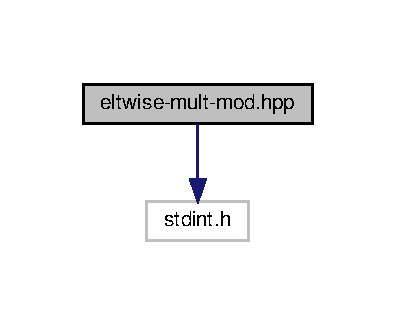
\includegraphics[width=190pt]{eltwise-mult-mod_8hpp__incl}
\end{center}
\end{figure}
This graph shows which files directly or indirectly include this file\+:
\nopagebreak
\begin{figure}[H]
\begin{center}
\leavevmode
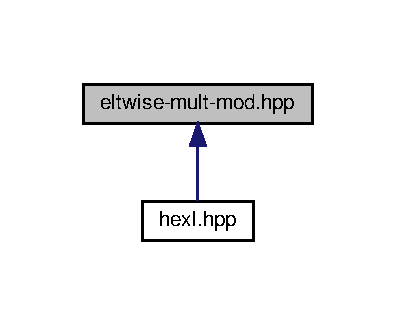
\includegraphics[width=190pt]{eltwise-mult-mod_8hpp__dep__incl}
\end{center}
\end{figure}
\subsection*{Namespaces}
\begin{DoxyCompactItemize}
\item 
 \hyperlink{namespaceintel}{intel}
\item 
 \hyperlink{namespaceintel_1_1hexl}{intel\+::hexl}
\end{DoxyCompactItemize}
\subsection*{Functions}
\begin{DoxyCompactItemize}
\item 
void \hyperlink{namespaceintel_1_1hexl_a705bc0321d937ae4d1f8d50279e3cff1}{intel\+::hexl\+::\+Eltwise\+Mult\+Mod} (uint64\+\_\+t $\ast$result, const uint64\+\_\+t $\ast$operand1, const uint64\+\_\+t $\ast$operand2, uint64\+\_\+t n, uint64\+\_\+t modulus, uint64\+\_\+t input\+\_\+mod\+\_\+factor)
\begin{DoxyCompactList}\small\item\em Multiplies two vectors elementwise with modular reduction. \end{DoxyCompactList}\end{DoxyCompactItemize}

\hypertarget{eltwise-reduce-mod_8hpp}{}\doxysection{/\+Users/fboemer/repos/\+D\+B\+I\+O/intel-\/hexl/hexl/include/hexl/eltwise/eltwise-\/reduce-\/mod.hpp File Reference}
\label{eltwise-reduce-mod_8hpp}\index{/Users/fboemer/repos/DBIO/intel-\/hexl/hexl/include/hexl/eltwise/eltwise-\/reduce-\/mod.hpp@{/Users/fboemer/repos/DBIO/intel-\/hexl/hexl/include/hexl/eltwise/eltwise-\/reduce-\/mod.hpp}}
{\ttfamily \#include $<$stdint.\+h$>$}\newline
\doxysubsection*{Namespaces}
\begin{DoxyCompactItemize}
\item 
 \mbox{\hyperlink{namespaceintel}{intel}}
\item 
 \mbox{\hyperlink{namespaceintel_1_1hexl}{intel\+::hexl}}
\end{DoxyCompactItemize}
\doxysubsection*{Functions}
\begin{DoxyCompactItemize}
\item 
void \mbox{\hyperlink{namespaceintel_1_1hexl_af3ddae165283841d495a322275baf5ee}{intel\+::hexl\+::\+Eltwise\+Reduce\+Mod}} (uint64\+\_\+t $\ast$result, const uint64\+\_\+t $\ast$operand, uint64\+\_\+t n, uint64\+\_\+t modulus, uint64\+\_\+t input\+\_\+mod\+\_\+factor, uint64\+\_\+t output\+\_\+mod\+\_\+factor)
\begin{DoxyCompactList}\small\item\em Performs elementwise modular reduction. \end{DoxyCompactList}\end{DoxyCompactItemize}

\hypertarget{eltwise-sub-mod_8hpp}{}\doxysection{/\+Users/fboemer/repos/\+D\+B\+I\+O/intel-\/hexl/hexl/include/hexl/eltwise/eltwise-\/sub-\/mod.hpp File Reference}
\label{eltwise-sub-mod_8hpp}\index{/Users/fboemer/repos/DBIO/intel-\/hexl/hexl/include/hexl/eltwise/eltwise-\/sub-\/mod.hpp@{/Users/fboemer/repos/DBIO/intel-\/hexl/hexl/include/hexl/eltwise/eltwise-\/sub-\/mod.hpp}}
{\ttfamily \#include $<$stdint.\+h$>$}\newline
\doxysubsection*{Namespaces}
\begin{DoxyCompactItemize}
\item 
 \mbox{\hyperlink{namespaceintel}{intel}}
\item 
 \mbox{\hyperlink{namespaceintel_1_1hexl}{intel\+::hexl}}
\end{DoxyCompactItemize}
\doxysubsection*{Functions}
\begin{DoxyCompactItemize}
\item 
void \mbox{\hyperlink{namespaceintel_1_1hexl_a6a45c30bc21b9b1e1410b23fce5424c8}{intel\+::hexl\+::\+Eltwise\+Sub\+Mod}} (uint64\+\_\+t $\ast$result, const uint64\+\_\+t $\ast$operand1, const uint64\+\_\+t $\ast$operand2, uint64\+\_\+t n, uint64\+\_\+t modulus)
\begin{DoxyCompactList}\small\item\em Subtracts two vectors elementwise with modular reduction. \end{DoxyCompactList}\item 
void \mbox{\hyperlink{namespaceintel_1_1hexl_abc13b8f383d3af6471a5261ee2213b40}{intel\+::hexl\+::\+Eltwise\+Sub\+Mod}} (uint64\+\_\+t $\ast$result, const uint64\+\_\+t $\ast$operand1, uint64\+\_\+t operand2, uint64\+\_\+t n, uint64\+\_\+t modulus)
\begin{DoxyCompactList}\small\item\em Subtracts a scalar from a vector elementwise with modular reduction. \end{DoxyCompactList}\end{DoxyCompactItemize}

\hypertarget{hexl_8hpp}{}\section{hexl.\+hpp File Reference}
\label{hexl_8hpp}\index{hexl.\+hpp@{hexl.\+hpp}}
{\ttfamily \#include \char`\"{}hexl/eltwise/eltwise-\/add-\/mod.\+hpp\char`\"{}}\newline
{\ttfamily \#include \char`\"{}hexl/eltwise/eltwise-\/cmp-\/add.\+hpp\char`\"{}}\newline
{\ttfamily \#include \char`\"{}hexl/eltwise/eltwise-\/cmp-\/sub-\/mod.\+hpp\char`\"{}}\newline
{\ttfamily \#include \char`\"{}hexl/eltwise/eltwise-\/fma-\/mod.\+hpp\char`\"{}}\newline
{\ttfamily \#include \char`\"{}hexl/eltwise/eltwise-\/mult-\/mod.\+hpp\char`\"{}}\newline
{\ttfamily \#include \char`\"{}hexl/eltwise/eltwise-\/reduce-\/mod.\+hpp\char`\"{}}\newline
{\ttfamily \#include \char`\"{}hexl/eltwise/eltwise-\/sub-\/mod.\+hpp\char`\"{}}\newline
{\ttfamily \#include \char`\"{}hexl/ntt/ntt.\+hpp\char`\"{}}\newline
{\ttfamily \#include \char`\"{}hexl/util/util.\+hpp\char`\"{}}\newline
Include dependency graph for hexl.\+hpp\+:
\nopagebreak
\begin{figure}[H]
\begin{center}
\leavevmode
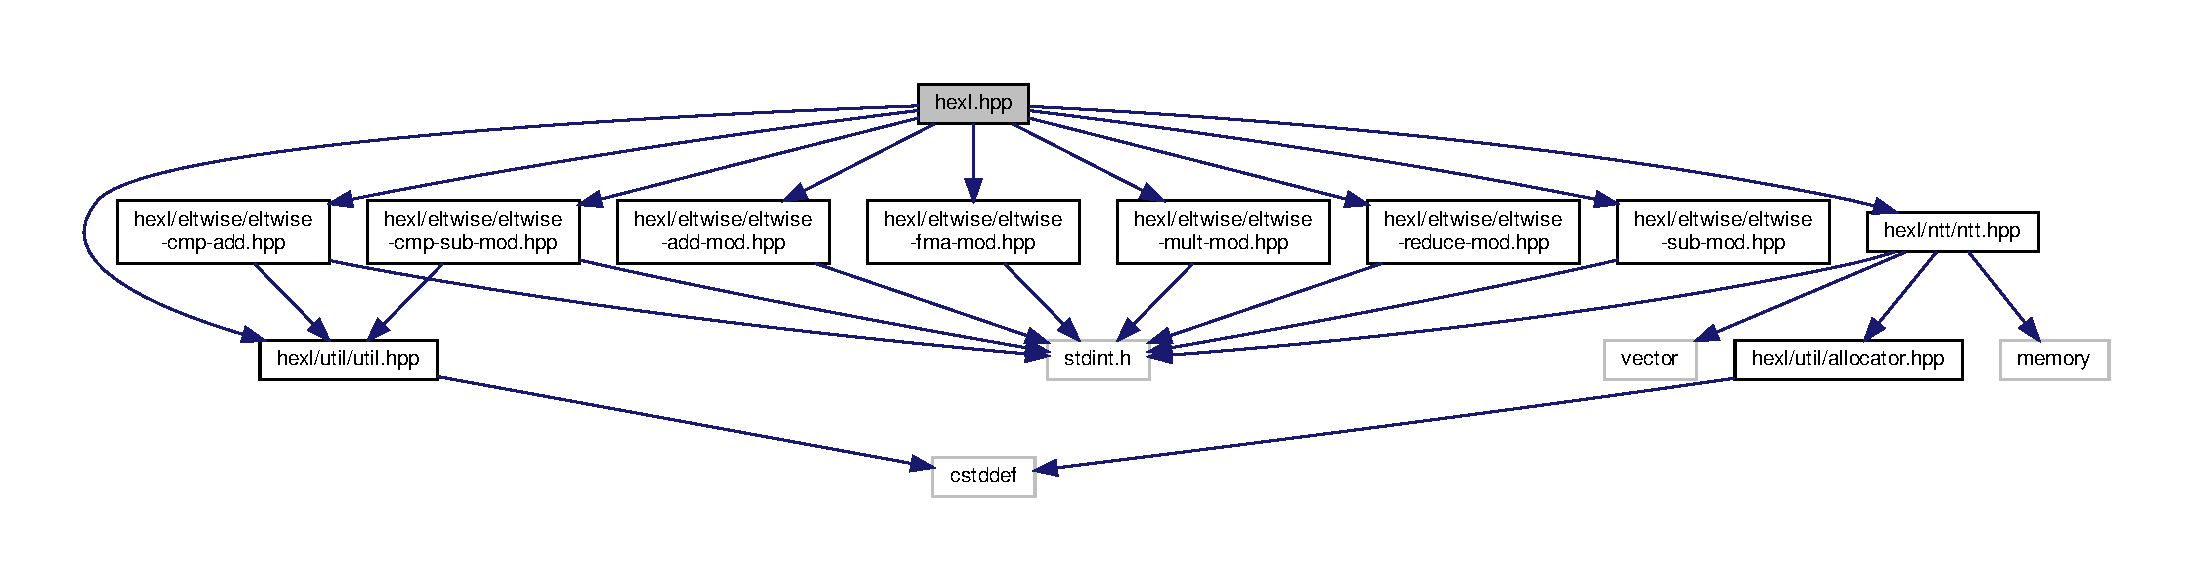
\includegraphics[width=350pt]{hexl_8hpp__incl}
\end{center}
\end{figure}

\hypertarget{ntt_8hpp}{}\doxysection{ntt.\+hpp File Reference}
\label{ntt_8hpp}\index{ntt.hpp@{ntt.hpp}}
{\ttfamily \#include $<$stdint.\+h$>$}\newline
{\ttfamily \#include $<$memory$>$}\newline
{\ttfamily \#include $<$vector$>$}\newline
\doxysubsection*{Classes}
\begin{DoxyCompactItemize}
\item 
class \mbox{\hyperlink{classintel_1_1hexl_1_1_n_t_t}{intel\+::hexl\+::\+NTT}}
\begin{DoxyCompactList}\small\item\em Performs negacyclic forward and inverse number-\/theoretic transform (\mbox{\hyperlink{classintel_1_1hexl_1_1_n_t_t}{NTT}}), commonly used in RLWE cryptography. \end{DoxyCompactList}\end{DoxyCompactItemize}
\doxysubsection*{Namespaces}
\begin{DoxyCompactItemize}
\item 
namespace \mbox{\hyperlink{namespaceintel}{intel}}
\item 
namespace \mbox{\hyperlink{namespaceintel_1_1hexl}{intel\+::hexl}}
\end{DoxyCompactItemize}

\hypertarget{README_8md}{}\section{R\+E\+A\+D\+M\+E.\+md File Reference}
\label{README_8md}\index{R\+E\+A\+D\+M\+E.\+md@{R\+E\+A\+D\+M\+E.\+md}}

\hypertarget{util_8hpp}{}\doxysection{util.\+hpp File Reference}
\label{util_8hpp}\index{util.hpp@{util.hpp}}
\doxysubsection*{Namespaces}
\begin{DoxyCompactItemize}
\item 
namespace \mbox{\hyperlink{namespaceintel}{intel}}
\item 
namespace \mbox{\hyperlink{namespaceintel_1_1hexl}{intel\+::hexl}}
\end{DoxyCompactItemize}
\doxysubsection*{Enumerations}
\begin{DoxyCompactItemize}
\item 
enum class \mbox{\hyperlink{namespaceintel_1_1hexl_abdcc9d2d5bb10fa95d5f143874508006}{intel\+::hexl\+::\+CMPINT}} \{ \newline
\mbox{\hyperlink{namespaceintel_1_1hexl_abdcc9d2d5bb10fa95d5f143874508006a2dcbad7477fd40561e8b8198f173bd47}{intel\+::hexl\+::\+EQ}} = 0
, \mbox{\hyperlink{namespaceintel_1_1hexl_abdcc9d2d5bb10fa95d5f143874508006ac562607189d77eb9dfb707464c1e7b0b}{intel\+::hexl\+::\+LT}} = 1
, \mbox{\hyperlink{namespaceintel_1_1hexl_abdcc9d2d5bb10fa95d5f143874508006acfe6055d2e0503be378bb63449ec7ba6}{intel\+::hexl\+::\+LE}} = 2
, \mbox{\hyperlink{namespaceintel_1_1hexl_abdcc9d2d5bb10fa95d5f143874508006a946003f97ccc52d5d3b54ac0ec31bbfc}{intel\+::hexl\+::\+FALSE}} = 3
, \newline
\mbox{\hyperlink{namespaceintel_1_1hexl_abdcc9d2d5bb10fa95d5f143874508006adc33066c3993e0d50896e533fd692ce0}{intel\+::hexl\+::\+NE}} = 4
, \mbox{\hyperlink{namespaceintel_1_1hexl_abdcc9d2d5bb10fa95d5f143874508006ad7d6a13c7b311ec8a3c9fcfb1919a2f8}{intel\+::hexl\+::\+NLT}} = 5
, \mbox{\hyperlink{namespaceintel_1_1hexl_abdcc9d2d5bb10fa95d5f143874508006aacd748f300c5d189c47807e2a9d6ea57}{intel\+::hexl\+::\+NLE}} = 6
, \mbox{\hyperlink{namespaceintel_1_1hexl_abdcc9d2d5bb10fa95d5f143874508006ac0d83f0b82a6b30de8811e69e6d95c61}{intel\+::hexl\+::\+TRUE}} = 7
 \}
\begin{DoxyCompactList}\small\item\em Represents binary operations between two boolean values. \end{DoxyCompactList}\end{DoxyCompactItemize}
\doxysubsection*{Functions}
\begin{DoxyCompactItemize}
\item 
CMPINT \mbox{\hyperlink{namespaceintel_1_1hexl_a8c654502a5e7fe2cfdd198f0fd920f2a}{intel\+::hexl\+::\+Not}} (CMPINT cmp)
\begin{DoxyCompactList}\small\item\em Returns the logical negation of a binary operation. \end{DoxyCompactList}\end{DoxyCompactItemize}

%--- End generated contents ---

% Index
\backmatter
\newpage
\phantomsection
\clearemptydoublepage
\addcontentsline{toc}{chapter}{Index}
\printindex

\end{document}
